%! Unidad 7 — La química del carbono (teoría, ejemplos resueltos, ejercicios por apartados, lectura, prácticas y situación de
%! aprendizaje)
%! Fuente: Fuentes/Quimica/Unidad 7 (capturas 557 —portada, mitad derecha— a 572 y solucionario). Texto reescrito; compuestos y
%!   datos de los ejercicios cambiados y recalculados.
%! Normas de nomenclatura: recomendaciones IUPAC 2013 (cadena principal = la más larga; localizadores delante de la terminación:
%!   but-1-eno, pent-1-en-4-ino). Masas atómicas: H 1; C 12; N 14; O 16; Cl 35,5. Triple enlace en \ch con «+» (\ch{CH+CH});
%!   en chemfig, «~». Estructuras ramificadas y anillos con chemfig (atom sep 1.8em en esta unidad).
%! Figuras en images/UD7/: nuevas en html/ (clasificacion_hidrocarburos, torre_destilacion), copiadas (PDF + SVG) de
%!   4ESO/images/UD4 (tetraedro, enlaces_cc, oxigenados, enlace_hidrogeno, aminas, polietileno) y de
%!   2BachQuimica/FigurasSVG/UD9_Quimica_Organica (enantiomeros = UD9_09_imagen_especular).

\sloppy % nombres largos sin guiones: se permite más espacio entre palabras (\fussy al final)
\setchemfig{atom sep=1.8em}

\section*{Para empezar: el elemento de la vida}
\addcontentsline{toc}{section}{Para empezar: el elemento de la vida}

Los seres vivos estamos hechos de glúcidos, lípidos, proteínas y ácidos nucleicos, y todas esas moléculas tienen un esqueleto de
átomos de \textbf{carbono}. Del carbono proceden también la gasolina y el gas natural, casi todos los plásticos, los medicamentos,
los colorantes, los perfumes o las fibras sintéticas de la ropa. Se conocen más de 24 millones de compuestos de carbono, muchísimos
más que de todos los demás elementos juntos (algo más de medio millón).

Pero el carbono es especial incluso solo: según cómo se unan sus átomos forma el \textbf{diamante}, el material natural más duro; el
\textbf{grafito} de los lápices; los \textbf{fullerenos}, moléculas con forma de balón; los \textbf{nanotubos} o el
\textbf{grafeno}, una lámina de un átomo de grosor que conduce la electricidad mejor que el cobre. En esta unidad veremos por qué
el carbono forma tantos compuestos, cómo se representan, cómo se nombran según las normas de la IUPAC y qué importancia tienen en la
industria y en la vida.

%========================================================================================
\section{Recuerda de la ESO}\label{sec:ud7-eso}
%========================================================================================

\paragraph{El átomo de carbono.} El carbono (\(Z = 6\)) tiene 6 protones y 6 electrones, cuatro de ellos en la capa de valencia.
Para completar el octeto forma \textbf{enlaces covalentes} compartiendo cuatro pares de electrones.

\paragraph{Enlaces entre carbonos.} Dos átomos de carbono pueden compartir un par de electrones (\textbf{enlace sencillo},
\ch{C-C}), dos pares (\textbf{enlace doble}, \ch{C=C}) o tres pares (\textbf{enlace triple}, \ch{C+C}). Así se forman
\textbf{cadenas} de átomos de carbono, que pueden ser muy largas.

\paragraph{Hidrocarburos.} Son los compuestos de carbono más sencillos: solo tienen carbono e hidrógeno. Los que solo tienen
enlaces sencillos son los \textbf{alcanos}, que se nombran con un prefijo que indica el número de carbonos y la terminación
\textbf{-ano}:

\begin{table}[H]
    \centering
    \caption{Los seis primeros alcanos de cadena lineal}
    \vspace{-5pt}
    \begin{tabular}{@{}clll@{}}
        \toprule
        \textbf{N.º de C} & \textbf{Nombre} & \textbf{Fórmula semidesarrollada} & \textbf{Fórmula molecular} \\
        \midrule
        1 & metano & \ch{CH4} & \ch{CH4} \\[3pt]
        2 & etano & \ch{CH3-CH3} & \ch{C2H6} \\[3pt]
        3 & propano & \ch{CH3-CH2-CH3} & \ch{C3H8} \\[3pt]
        4 & butano & \ch{CH3-CH2-CH2-CH3} & \ch{C4H10} \\[3pt]
        5 & pentano & \ch{CH3-CH2-CH2-CH2-CH3} & \ch{C5H12} \\[3pt]
        6 & hexano & \ch{CH3-CH2-CH2-CH2-CH2-CH3} & \ch{C6H14} \\
        \bottomrule
    \end{tabular}
    \label{tab:ud7-alcanos-eso}
\end{table}

\begin{exercise}
    Escribe la fórmula desarrollada del propano y la semidesarrollada del heptano. ¿Cuántos enlaces \ch{C-H} y \ch{C-C} hay en
    cada uno?
    \begin{solu}
        \textcolor{blue}{Propano:} \(\chemfig{H-C(-[2]H)(-[6]H)-C(-[2]H)(-[6]H)-C(-[2]H)(-[6]H)-H}\):
        \textcolor{red}{8 enlaces \ch{C-H} y 2 \ch{C-C}}. \textcolor{blue}{Heptano:} \ch{CH3-CH2-CH2-CH2-CH2-CH2-CH3}
        (\ch{C7H16}): \textcolor{red}{16 enlaces \ch{C-H} y 6 \ch{C-C}}. En general, un alcano lineal de \(n\) carbonos tiene
        \(2n + 2\) enlaces \ch{C-H} y \(n - 1\) enlaces \ch{C-C}.
    \end{solu}
\end{exercise}

\begin{exercise}
    En el etano, el eteno y el etino, ¿cuántos pares de electrones comparte cada carbono con el otro carbono? ¿Con cuántos
    hidrógenos se une cada carbono? Escribe sus fórmulas semidesarrolladas.
    \begin{solu}
        \textcolor{red}{Etano, \ch{CH3-CH3}: 1 par y 3 H por carbono. Eteno, \ch{CH2=CH2}: 2 pares y 2 H. Etino, \ch{CH+CH}:
        3 pares y 1 H.} En los tres casos cada carbono comparte cuatro pares de electrones en total.
    \end{solu}
\end{exercise}

%========================================================================================
\section{De la química orgánica a la química del carbono}\label{sec:ud7-historia}
%========================================================================================

Desde la Antigüedad se aprovechan procesos en los que intervienen sustancias de origen vivo: la fermentación del vino y la cerveza,
la fabricación de jabón con grasas o el curtido de las pieles con \textbf{taninos}, sustancias vegetales que se unen a las proteínas
del cuero y lo hacen resistente a la putrefacción. En 1807, el sueco \textbf{J. J. Berzelius} dividió las sustancias en dos grandes
grupos:
\begin{itemize}
    \item \textbf{orgánicas}, producidas por los seres vivos, y
    \item \textbf{inorgánicas}, propias de la materia no viva.
\end{itemize}
Se pensaba que las sustancias orgánicas solo podían formarse gracias a una \emph{fuerza vital} propia de los seres vivos y que era
imposible obtenerlas en el laboratorio (\textbf{vitalismo}). En 1828, el alemán \textbf{F. Wöhler} obtuvo \textbf{urea}, una
sustancia presente en la orina, calentando cianato de amonio, una sal inorgánica:
\[ \ch{NH4OCN ->[\(\Delta\)] (NH2)2CO} \]
Con el tiempo se sintetizaron muchas otras sustancias orgánicas y la teoría de la fuerza vital se abandonó. Lo que sí tienen en
común todas las sustancias orgánicas es que contienen \textbf{carbono}.

\begin{definition}[Química orgánica o química del carbono]
    Es la rama de la química que estudia los compuestos del carbono. Algunas sustancias con carbono, como el \ch{CO}, el \ch{CO2},
    el ácido carbónico, los carbonatos y los cianuros, se estudian tradicionalmente con la química inorgánica.
\end{definition}

Los compuestos orgánicos suelen arder con facilidad (\textbf{combustión}), desprendiendo energía, y se descomponen o transforman
con la luz o el calor. Muchos son poco solubles en agua y tienen puntos de fusión y ebullición bajos, porque están formados por
moléculas.

\subsection{El átomo de carbono}

¿Qué tiene de especial el carbono para que exista una rama entera de la química dedicada a él? Su configuración electrónica es
\conf{1s^2\,2s^2\,2p^2}: está en el período 2 y el grupo 14, es un no metal y tiene una electronegatividad intermedia (2,5 en la
escala de Pauling). Con esta configuración solo tendría dos electrones desapareados:
\[ \underset{2s}{\orbcaja{\uparrow\downarrow}} \quad \underset{2p}{\orbcaja{\uparrow}\orbcaja{\uparrow}\orbcaja{}} \]
Sin embargo, la energía de los subniveles 2s y 2p es parecida, y uno de los electrones 2s puede \textbf{promocionar} al orbital 2p
vacío. Quedan así cuatro electrones desapareados, que permiten formar \textbf{cuatro enlaces covalentes}: es la
\textbf{tetravalencia} del carbono.
\[ \underset{2s}{\orbcaja{\uparrow}} \quad \underset{2p}{\orbcaja{\uparrow}\orbcaja{\uparrow}\orbcaja{\uparrow}} \]
La energía que cuesta la promoción se recupera con creces al formar dos enlaces más.

\paragraph{Orbitales híbridos.} Los cuatro enlaces del metano, \ch{CH4}, son idénticos y forman entre sí ángulos de
\ang{109.5}: apuntan a los vértices de un tetraedro regular. Se explica suponiendo que el orbital 2s y los tres 2p se combinan y dan
cuatro \textbf{orbitales híbridos} iguales, llamados \(sp^3\). Los pares de electrones de los enlaces se alejan lo más posible para
repelerse lo menos posible (figura~\ref{fig:ud7-tetraedro}).

\begin{figure}[H]
    \centering
    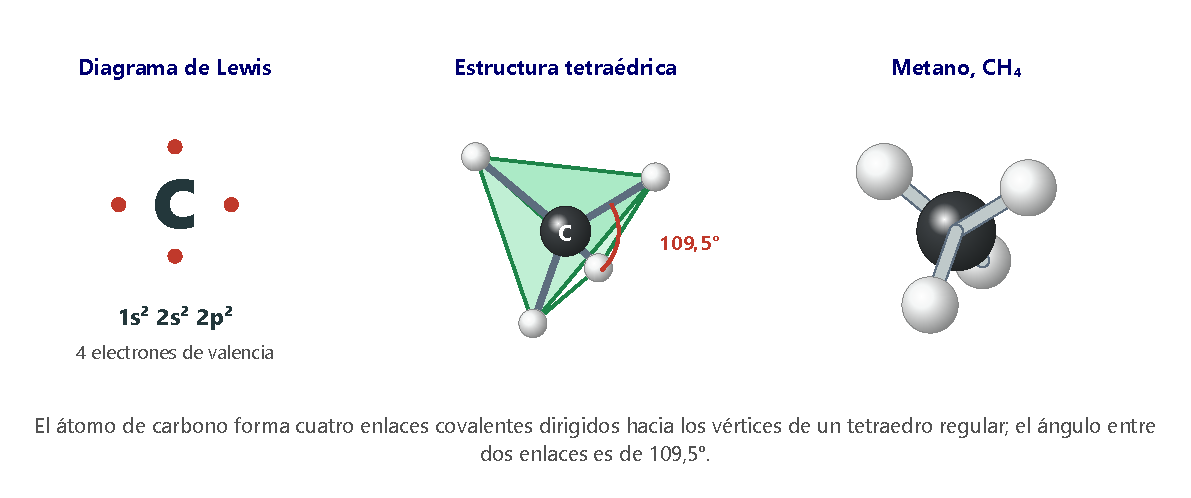
\includegraphics[width=0.85\textwidth]{images/UD7/tetraedro}
    \caption{El carbono forma cuatro enlaces dirigidos hacia los vértices de un tetraedro regular.}
    \label{fig:ud7-tetraedro}
\end{figure}

Según los enlaces que forme, el carbono presenta tres geometrías (figura~\ref{fig:ud7-enlaces}):

\begin{table}[H]
    \centering
    \caption{Tipos de carbono según sus enlaces}
    \vspace{-5pt}
    \begin{tabular}{@{}L{3.8cm}cccl@{}}
        \toprule
        \textbf{Enlaces del carbono} & \textbf{Hibridación} & \textbf{Geometría} & \textbf{Ángulo} & \textbf{Ejemplo} \\
        \midrule
        Cuatro sencillos & \(sp^3\) & tetraédrica & \ang{109.5} & etano, \ch{CH3-CH3} \\[3pt]
        Uno doble y dos sencillos & \(sp^2\) & plana triangular & \ang{120} & eteno, \ch{CH2=CH2} \\[3pt]
        Uno triple y uno sencillo, o dos dobles & \(sp\) & lineal & \ang{180} & etino, \ch{CH+CH} \\
        \bottomrule
    \end{tabular}
    \label{tab:ud7-hibridacion}
\end{table}

\begin{figure}[H]
    \centering
    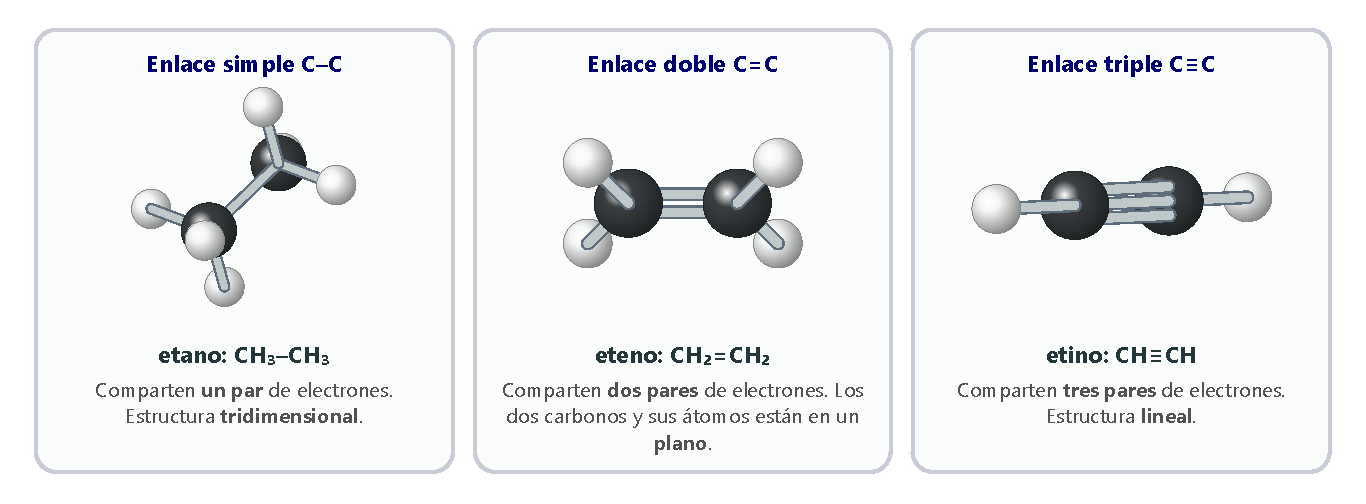
\includegraphics[width=0.85\textwidth]{images/UD7/enlaces_cc}
    \caption{Enlaces sencillo, doble y triple entre átomos de carbono.}
    \label{fig:ud7-enlaces}
\end{figure}

\subsection{Cadenas, enlaces y heteroátomos}

El enlace covalente \ch{C-C} es muy fuerte, y por eso los átomos de carbono pueden unirse entre sí formando \textbf{cadenas}
\textbf{abiertas} (lineales o ramificadas) o \textbf{cerradas} (anillos), a veces de miles de átomos:
\[ \underset{\text{lineal}}{\chemfig{C-C-C-C}} \qquad\quad
   \underset{\text{ramificada}}{\chemfig{C-C(-[6]C)-C-C}} \qquad\quad
   \underset{\text{cerrada}}{\chemfig{C*5(-C-C-C-C-)}} \]
Los compuestos que solo tienen enlaces sencillos entre carbonos son \textbf{saturados}; los que tienen algún enlace doble o triple
(enlaces múltiples o \textbf{insaturaciones}) son \textbf{insaturados}.

Además de hidrógeno, los compuestos del carbono pueden contener oxígeno, nitrógeno y, en menor cantidad, halógenos, azufre, fósforo e
incluso metales. Cualquier átomo distinto del C y el H en un compuesto orgánico es un \textbf{heteroátomo}.

\paragraph{Tipos de carbono.} Un carbono es \textbf{primario} si está unido a un solo carbono, \textbf{secundario} si está unido a
dos, \textbf{terciario} si está unido a tres y \textbf{cuaternario} si está unido a cuatro, sean los enlaces sencillos o múltiples.
En el 2,2,4-trimetilpentano, por ejemplo,
\[ \chemfig{\underset{1^\circ}{CH_3}-\underset{4^\circ}{C}(-[2]CH_3)(-[6]CH_3)-\underset{2^\circ}{CH_2}-\underset{3^\circ}{CH}(-[6]CH_3)-CH_3} \]

\begin{exercise}
    Indica la hibridación de cada carbono y los ángulos de enlace aproximados en el compuesto \ch{CH2=CH-CH2-C+CH}.
    \begin{solu}
        Numerando de izquierda a derecha: \textcolor{red}{C1 y C2, \(sp^2\) (\ang{120}); C3, \(sp^3\) (\ang{109.5}); C4 y C5,
        \(sp\) (\ang{180})}.
    \end{solu}
\end{exercise}

\begin{exercise}
    Clasifica los carbonos del compuesto \chemfig{CH_3-C(-[2]CH_3)(-[6]CH_3)-CH_2-CH(-[6]CH_3)-CH_3} en primarios, secundarios,
    terciarios y cuaternarios.
    \begin{solu}
        \textcolor{red}{5 primarios} (los cinco \ch{CH3}), \textcolor{red}{1 secundario} (el \ch{CH2}), \textcolor{red}{1
        terciario} (el \ch{CH}) y \textcolor{red}{1 cuaternario} (el C unido a cuatro carbonos). En total, 8 carbonos: es el
        2,2,4-trimetilpentano, \ch{C8H18}, el «isooctano» que se usa como referencia del octanaje de las gasolinas.
    \end{solu}
\end{exercise}

\begin{exercise}
    ¿Verdadero o falso? Justifica. a) Todos los compuestos con carbono son orgánicos. b) Wöhler demostró que las sustancias
    orgánicas pueden obtenerse a partir de sustancias inorgánicas. c) En el etino los átomos están en línea recta. d) Un compuesto
    con un enlace triple es saturado.
    \begin{solu}
        a) \textcolor{red}{Falso}: el \ch{CO}, el \ch{CO2} o los carbonatos son inorgánicos. b) \textcolor{red}{Verdadero}: sintetizó
        urea a partir de cianato de amonio. c) \textcolor{red}{Verdadero}: los carbonos son \(sp\) y los ángulos son de
        \ang{180}. d) \textcolor{red}{Falso}: es insaturado.
    \end{solu}
\end{exercise}

%========================================================================================
\section{Las fórmulas de los compuestos del carbono}\label{sec:ud7-formulas}
%========================================================================================

Las propiedades de una sustancia orgánica dependen no solo de los átomos que la forman, sino de \textbf{cómo están unidos}. Por eso,
además de las fórmulas empírica y molecular que ya conoces, necesitamos fórmulas que muestren los enlaces.

\subsection{Fórmulas empírica y molecular}

\begin{definition}[Fórmula empírica y fórmula molecular]
    La \textbf{fórmula empírica} indica la \textbf{proporción} más sencilla en que están los átomos de cada elemento. La
    \textbf{fórmula molecular} indica el \textbf{número real} de átomos de cada elemento en una molécula; es un múltiplo entero de
    la empírica y se obtiene con ella y la \textbf{masa molar}.
\end{definition}

El acetileno (\ch{C2H2}) y el benceno (\ch{C6H6}) tienen la misma fórmula empírica, \ch{CH}, pero distinta fórmula molecular. La
fórmula empírica de un compuesto orgánico se determina en el laboratorio quemando una masa conocida y midiendo el \ch{CO2} y el
\ch{H2O} que se forman: \textbf{todo el C pasa al \ch{CO2} y todo el H al \ch{H2O}}. La masa molar se obtiene con la densidad del
gas, la ecuación de los gases o las propiedades coligativas (unidades 1 y 2).

\begin{example}
    \textbf{Fórmula de un hidrocarburo por combustión.} Al quemar por completo un hidrocarburo se obtienen \qty{26.4}{\gram} de
    \ch{CO2} y \qty{13.5}{\gram} de \ch{H2O}. Su masa molar es \qty{58}{\gram\per\mol}. Halla sus fórmulas empírica y molecular.

    \textbf{Solución.} \(\ch{C_xH_y + O2 -> CO2 + H2O}\); \(M(\ch{CO2}) = \qty{44}{\gram\per\mol}\), \(M(\ch{H2O}) =
    \qty{18}{\gram\per\mol}\).
    \[ n(\ch{C}) = \frac{26{,}4}{44} = \qty{0.600}{\mol} \qquad n(\ch{H}) = 2 \cdot \frac{13{,}5}{18} = \qty{1.50}{\mol} \]
    Dividimos por el menor: \(\dfrac{0{,}600}{0{,}600} = 1\); \(\dfrac{1{,}50}{0{,}600} = 2{,}5\). Multiplicando por 2 para tener
    enteros: \(\ch{C2H5}\), con masa \(2 \cdot 12 + 5 = 29\). Como \(58/29 = 2\), la fórmula molecular es \(\ch{(C2H5)2} =
    \ch{C4H10}\) (butano o metilpropano).
\end{example}

\begin{example}
    \textbf{Compuesto con oxígeno.} Una muestra de \qty{2.30}{\gram} de un compuesto de C, H y O produce al arder \qty{4.40}{\gram}
    de \ch{CO2} y \qty{2.70}{\gram} de \ch{H2O}. Una masa de \qty{0.46}{\gram} de su vapor ocupa \qty{306}{\mL} a
    \qty{100}{\degreeCelsius} y \qty{1}{\atm}. Halla su fórmula molecular.

    \textbf{Solución.} \(m(\ch{C}) = 4{,}40 \cdot \frac{12}{44} = \qty{1.20}{\gram}\) (\(\qty{0.100}{\mol}\));
    \(m(\ch{H}) = 2{,}70 \cdot \frac{2}{18} = \qty{0.300}{\gram}\) (\(\qty{0.300}{\mol}\)). El oxígeno es lo que falta:
    \(m(\ch{O}) = 2{,}30 - 1{,}20 - 0{,}300 = \qty{0.80}{\gram}\) (\(\qty{0.050}{\mol}\)). Proporción
    \(0{,}100 : 0{,}300 : 0{,}050 = 2 : 6 : 1\): fórmula empírica \ch{C2H6O} (\(M = 46\)). Con los gases:
    \[ M = \frac{m\,R\,T}{p\,V} = \frac{0{,}46 \cdot 0{,}082 \cdot 373}{1 \cdot 0{,}306} = \qty{46}{\gram\per\mol} \]
    La fórmula molecular es \ch{C2H6O}: puede ser el etanol, \ch{CH3-CH2OH}, o el dimetil éter, \ch{CH3-O-CH3}. Para saber cuál
    es hace falta otro dato, como su punto de ebullición.
\end{example}

\begin{remark}
    La estructura exacta de un compuesto se determina con técnicas como la espectroscopía infrarroja, la resonancia magnética
    nuclear (RMN), la espectrometría de masas o la difracción de rayos X.
\end{remark}

\subsection{Fórmulas estructurales}

\begin{table}[H]
    \centering
    \caption{Tipos de fórmulas estructurales, con el ejemplo del butano}
    \vspace{-5pt}
    \begin{tabular}{@{}L{2.65cm}L{6cm}C{5.35cm}@{}}
        \toprule
        \textbf{Fórmula} & \textbf{Qué representa} & \textbf{Butano} \\
        \midrule
        Desarrollada & Todos los átomos y todos los enlaces, en el plano. No informa de la disposición en el espacio. &
        \chemfig{H-C(-[2]H)(-[6]H)-C(-[2]H)(-[6]H)-C(-[2]H)(-[6]H)-C(-[2]H)(-[6]H)-H} \\[3pt]
        Semidesarrollada & Solo los enlaces entre carbonos (y con los grupos funcionales); los H se agrupan con su carbono. &
        \ch{CH3-CH2-CH2-CH3} o \ch{CH3-(CH2)2-CH3} \\[3pt]
        En esqueleto (zigzag) & Cada vértice y cada extremo es un carbono; los H unidos a C no se escriben. &
        \chemfig{-[:30]-[:-30]-[:30]} \\[3pt]
        Geométrica o tridimensional & La disposición en el espacio: las cuñas gruesas salen del papel y las discontinuas se
        alejan. & \chemfig{H_3C-C(<[2]H)(<:[6]H)-C(<[2]H)(<:[6]H)-CH_3} \\
        \bottomrule
    \end{tabular}
    \label{tab:ud7-formulas}
\end{table}

Los \textbf{modelos moleculares} de bolas y varillas o de esferas permiten ver la forma de la molécula, los ángulos de enlace y el
tamaño relativo de los átomos.

\begin{exercise}
    Al quemar un hidrocarburo gaseoso se obtienen \qty{13.2}{\gram} de \ch{CO2} y \qty{5.4}{\gram} de \ch{H2O}. Si su densidad en
    condiciones normales es \qty{1.875}{\gram\per\litre}, halla: a) su fórmula empírica; b) su fórmula molecular.
    \begin{solu}
        \textcolor{blue}{\(n(\ch{C}) = 13{,}2/44 = \qty{0.30}{\mol}\); \(n(\ch{H}) = 2 \cdot 5{,}4/18 = \qty{0.60}{\mol}\); proporción
        1 : 2.} a) \textcolor{red}{\ch{CH2}}. b) \textcolor{blue}{\(M = 1{,}875 \cdot 22{,}4 = \qty{42}{\gram\per\mol}\); \(42/14 = 3\).}
        \textcolor{red}{\ch{C3H6}}.
    \end{solu}
\end{exercise}

\begin{exercise}
    Al quemar \qty{1.80}{\gram} de un azúcar formado por C, H y O se obtienen \qty{2.64}{\gram} de \ch{CO2} y \qty{1.08}{\gram} de
    \ch{H2O}. Su masa molar es \qty{180}{\gram\per\mol}. Halla sus fórmulas empírica y molecular.
    \begin{solu}
        \textcolor{blue}{\(m(\ch{C}) = 2{,}64 \cdot 12/44 = \qty{0.72}{\gram}\) (\qty{0.060}{\mol}); \(m(\ch{H}) = 1{,}08 \cdot 2/18 =
        \qty{0.12}{\gram}\) (\qty{0.12}{\mol}); \(m(\ch{O}) = 1{,}80 - 0{,}72 - 0{,}12 = \qty{0.96}{\gram}\) (\qty{0.060}{\mol}).
        Proporción 1 : 2 : 1.} Empírica \textcolor{red}{\ch{CH2O}} (\(M = 30\)); \(180/30 = 6\): molecular
        \textcolor{red}{\ch{C6H12O6}} (glucosa o fructosa).
    \end{solu}
\end{exercise}

\begin{exercise}
    Un hidrocarburo contiene un 85,7\,\% de carbono. Una muestra de \qty{0.70}{\gram} de su vapor ocupa \qty{224}{\mL} en
    condiciones normales. Halla su fórmula molecular.
    \begin{solu}
        \textcolor{blue}{En \qty{100}{\gram}: \(85{,}7/12 = \qty{7.14}{\mol}\) de C y \(14{,}3/1 = \qty{14.3}{\mol}\) de H: proporción
        1 : 2, \ch{CH2}. \(n = 0{,}224/22{,}4 = \qty{0.0100}{\mol}\); \(M = 0{,}70/0{,}0100 = \qty{70}{\gram\per\mol}\); \(70/14 = 5\).}
        \textcolor{red}{\ch{C5H10}}.
    \end{solu}
\end{exercise}

\begin{exercise}
    Escribe la fórmula semidesarrollada y la molecular de los compuestos representados en esqueleto: a) \chemfig{-[:30]-[:-30]-[:30]-[:-30]};
    b) \chemfig{-[:30]=[:-30]-[:30]}; c) \chemfig{-[:30]-[:-30](-[6])-[:30]}.
    \begin{solu}
        a) \textcolor{red}{\ch{CH3-CH2-CH2-CH2-CH3}, \ch{C5H12}} (pentano). b) \textcolor{red}{\ch{CH3-CH=CH-CH3}, \ch{C4H8}}
        (but-2-eno). c) \textcolor{red}{\chemfig{CH_3-CH_2-CH(-[6]CH_3)-CH_3}, \ch{C5H12}} (2-metilbutano).
    \end{solu}
\end{exercise}

%========================================================================================
\section{Los compuestos del carbono: generalidades}\label{sec:ud7-generalidades}
%========================================================================================

\subsection{Estructura de los compuestos orgánicos}

\begin{definition}[Grupo funcional, familia y serie homóloga]
    Un \textbf{grupo funcional} es un átomo o grupo de átomos responsable del comportamiento químico de la sustancia: le da sus
    \textbf{propiedades características}. Los compuestos con el mismo grupo funcional forman una \textbf{familia} (por ejemplo, los
    alcoholes, con el grupo \ch{-OH}). Dentro de una familia, los compuestos que solo se diferencian en el número de grupos
    \ch{-CH2-} forman una \textbf{serie homóloga}.
\end{definition}

El etanol (\ch{CH3-CH2OH}), el butan-1-ol (\ch{CH3-CH2-CH2-CH2OH}) y el fenol (\ch{C6H5OH}) son de la misma familia, porque tienen
el grupo \ch{-OH}; además, el etanol y el butan-1-ol pertenecen a la misma serie homóloga.

\begin{itemize}
    \item La \textbf{cadena principal} es la cadena de átomos de carbono que se toma como base para el nombre. Si hay grupos
    funcionales, debe contener el \textbf{grupo funcional principal}.
    \item Los \textbf{sustituyentes} son las cadenas laterales (\textbf{ramificaciones}) y los grupos funcionales que no son el
    principal.
    \item Un \textbf{radical} (R) es un grupo de átomos que tiene un electrón desapareado, normalmente porque ha perdido un hidrógeno.
    Los radicales libres son inestables y muy reactivos; como sustituyentes, se unen a la cadena principal por ese electrón.
\end{itemize}

\subsection{Clasificación de los compuestos orgánicos}

\begin{table}[H]
    \centering
    \caption{Clasificación de los compuestos orgánicos que estudiaremos}
    \vspace{-5pt}
    \begin{tabular}{@{}L{5cm}L{4.5cm}L{4.5cm}@{}}
        \toprule
        \textbf{Hidrocarburos} (solo C y H) & \textbf{Compuestos oxigenados} & \textbf{Compuestos nitrogenados} \\
        \midrule
        Alifáticos de cadena abierta: alcanos, alquenos y alquinos & Alcoholes y fenoles & Aminas \\[3pt]
        Alifáticos de cadena cerrada: cicloalcanos, cicloalquenos y cicloalquinos & Éteres & Amidas \\[3pt]
        Aromáticos: benceno y derivados & Aldehídos y cetonas & Nitrilos \\[3pt]
        (Derivados halogenados) & Ácidos carboxílicos, ésteres y sales & \\
        \bottomrule
    \end{tabular}
    \label{tab:ud7-clasificacion}
\end{table}

Los hidrocarburos son el «esqueleto» del resto de los compuestos, y por eso empezaremos por ellos.

\begin{remark}
    Los primeros compuestos orgánicos recibieron nombres según su origen: el ácido \textbf{fórmico} se obtuvo de las hormigas
    (\emph{formica}, en latín), el ácido \textbf{láctico} de la leche y la \textbf{cadaverina}, de la descomposición de los
    cadáveres. Con millones de compuestos hace falta una nomenclatura \textbf{sistemática}, cuyas normas fija la \textbf{IUPAC}
    (Unión Internacional de Química Pura y Aplicada). Algunos nombres tradicionales, como acetona, ácido acético o benceno, siguen
    aceptados.
\end{remark}

\subsection{Prefijos que indican el número de carbonos}

\begin{table}[H]
    \centering
    \caption{Prefijos para el número de carbonos de una cadena}
    \vspace{-5pt}
    \begin{tabular}{@{}clclcl@{}}
        \toprule
        \textbf{N.º de C} & \textbf{Prefijo} & \textbf{N.º de C} & \textbf{Prefijo} & \textbf{N.º de C} & \textbf{Prefijo} \\
        \midrule
        1 & met- & 6 & hex- & 11 & undec- \\[3pt]
        2 & et- & 7 & hept- & 12 & dodec- \\[3pt]
        3 & prop- & 8 & oct- & 13 & tridec- \\[3pt]
        4 & but- & 9 & non- & 14 & tetradec- \\[3pt]
        5 & pent- & 10 & dec- & 20 & icos- \\
        \bottomrule
    \end{tabular}
    \label{tab:ud7-prefijos}
\end{table}

\paragraph{Reglas generales de la nomenclatura.}
\begin{itemize}
    \item Los enlaces múltiples se indican con las terminaciones \textbf{-en-} (doble) e \textbf{-in-} (triple).
    \item El grupo funcional principal se indica con un \textbf{sufijo}; los demás grupos funcionales, con un \textbf{prefijo}.
    \item La posición de los sustituyentes, los enlaces múltiples y el grupo principal se indica con números o
    \textbf{localizadores}, que se colocan \textbf{delante} de lo que señalan, separados por un \textbf{guion}: but-1-eno,
    2-metilpropano. Los números se separan entre sí con comas: 2,3-dimetilbutano.
    \item Si hay varios sustituyentes iguales se usan los prefijos \textbf{di-}, \textbf{tri-}, \textbf{tetra-}\ldots Los
    sustituyentes distintos se nombran por \textbf{orden alfabético}, sin tener en cuenta esos prefijos multiplicadores.
\end{itemize}

\subsection{Prioridad de los grupos funcionales}

Si un compuesto tiene varios grupos funcionales, el principal (el que se nombra como sufijo) es el de mayor prioridad según este
orden:

\begin{table}[H]
    \centering
    \caption{Grupos funcionales por orden de prioridad decreciente}
    \vspace{-5pt}
    \begin{tabular}{@{}clcll@{}}
        \toprule
        \textbf{Orden} & \textbf{Función} & \textbf{Grupo} & \makecell{\textbf{Sufijo}\\\textbf{(principal)}} & \makecell{\textbf{Prefijo}\\\textbf{(sustituyente)}} \\
        \midrule
        1 & Ácido carboxílico & \ch{-COOH} & ácido \ldots-oico & carboxi- \\[3pt]
        2 & Éster & \ch{-COO-R} & \ldots-oato de \ldots-ilo & (alcoxicarbonil-) \\[3pt]
        3 & Amida & \ch{-CONH2} & -amida & carbamoil- \\[3pt]
        4 & Nitrilo & \ch{-C+N} & -nitrilo & ciano- \\[3pt]
        5 & Aldehído & \ch{-CHO} & -al & formil- u oxo- \\[3pt]
        6 & Cetona & \ch{-CO-} & -ona & oxo- \\[3pt]
        7 & Alcohol & \ch{-OH} & -ol & hidroxi- \\[3pt]
        8 & Amina & \ch{-NH2} & -amina & amino- \\[3pt]
        9 & Éter & \ch{-O-} & (\ldots éter) & alcoxi- (metoxi-\ldots) \\
        \midrule
        — & Halógeno & \ch{-X} & — & fluoro-, cloro-, bromo-, yodo- \\[3pt]
        — & Radical alquilo & \ch{-R} & — & metil-, etil-\ldots \\
        \bottomrule
    \end{tabular}
    \label{tab:ud7-prioridad}
\end{table}

En los grupos \ch{-COOH}, \ch{-CONH2}, \ch{-C+N} y \ch{-CHO} el carbono del grupo forma parte de la cadena principal y se cuenta
en el nombre: \ch{CH3-COOH} es el ácido \emph{etanoico}, con dos carbonos. Los halógenos y los radicales alquilo nunca son grupo
principal: siempre se nombran como prefijos.

\begin{definition}[Cómo nombrar un compuesto orgánico]
    \leavevmode % el título de la definición en su propia línea, la lista debajo
    \begin{enumerate}
        \item Identifica el \textbf{grupo funcional principal}, que se nombrará con su \textbf{sufijo}.
        \item Elige la \textbf{cadena principal}: la que contiene el grupo principal y, entre ellas, la más larga.
        \item \textbf{Numera} la cadena dando al grupo principal el localizador más bajo posible; después, a los enlaces múltiples y,
        por último, a los sustituyentes.
        \item Nombra los \textbf{sustituyentes} con sus prefijos y localizadores, por orden alfabético.
        \item Nombra la cadena principal con el prefijo del número de carbonos, los enlaces múltiples (-an-, -en-, -in-) y el sufijo del
        grupo principal.
    \end{enumerate}
    Para \textbf{formular}: dibuja la cadena principal, numérala, coloca los enlaces múltiples, los grupos funcionales y los
    sustituyentes y, al final, completa con hidrógenos hasta que cada carbono tenga cuatro enlaces.
\end{definition}

\begin{example}
    \textbf{Analizar un nombre.} Explica qué indica cada parte del nombre \emph{ácido 3-hidroxi-6-metilhept-4-enoico} y formula
    el compuesto.

    \textbf{Solución.}
    \begin{itemize}
        \item \emph{ácido \ldots-oico}: el grupo principal es \ch{-COOH}; su carbono es el C1.
        \item \emph{hept-}: la cadena principal tiene 7 carbonos.
        \item \emph{-4-en-}: hay un doble enlace entre los carbonos 4 y 5.
        \item \emph{3-hidroxi}: un grupo \ch{-OH} en el C3; \emph{6-metil}: un radical \ch{-CH3} en el C6 (los sustituyentes van
        en orden alfabético: h antes que m).
    \end{itemize}
    \[ \chemfig{CH_3-CH(-[6]CH_3)-CH=CH-CH(-[6]OH)-CH_2-COOH} \]
\end{example}

\begin{exercise}
    Indica el grupo funcional y la familia de cada compuesto: a) \ch{CH3-CH2-CHO}; b) \ch{CH3-CO-CH3}; c) \ch{CH3-CH2-COOH};
    d) \ch{CH3-NH-CH3}; e) \ch{CH3-COO-CH3}; f) \ch{CH3-O-CH2-CH3}; g) \ch{CH3-CHOH-CH3}; h) \ch{CH3-CO-NH2}.
    \begin{solu}
        a) \textcolor{red}{\ch{-CHO}, aldehído}; b) \textcolor{red}{\ch{-CO-}, cetona}; c) \textcolor{red}{\ch{-COOH}, ácido
        carboxílico}; d) \textcolor{red}{\ch{-NH-}, amina} (secundaria); e) \textcolor{red}{\ch{-COO-}, éster}; f)
        \textcolor{red}{\ch{-O-}, éter}; g) \textcolor{red}{\ch{-OH}, alcohol}; h) \textcolor{red}{\ch{-CONH2}, amida}.
    \end{solu}
\end{exercise}

\begin{exercise}
    ¿Cuáles de estos compuestos pertenecen a la misma serie homóloga? \ch{CH3OH}, \ch{CH3-CH2-CH2OH}, \ch{CH3-O-CH3},
    \ch{CH3-CH2-CH2-CH2OH}, \ch{CH3-CHO}, \ch{CH3-CH2OH}.
    \begin{solu}
        \textcolor{red}{\ch{CH3OH}, \ch{CH3-CH2OH}, \ch{CH3-CH2-CH2OH} y \ch{CH3-CH2-CH2-CH2OH}}: son alcoholes con el \ch{-OH} en un
        extremo y solo se diferencian en grupos \ch{-CH2-}. El \ch{CH3-O-CH3} es un éter y el \ch{CH3-CHO}, un aldehído.
    \end{solu}
\end{exercise}

\begin{exercise}
    Indica el grupo principal, el número de carbonos de la cadena principal, los enlaces múltiples y los sustituyentes de:
    a) hepta-1,6-diin-4-ol; b) ácido 3-hidroxibutanoico; c) 2,3-dimetilpent-4-enal; d) 4-etil-6-metilhept-3-en-2-ona.
    \begin{solu}
        a) \textcolor{red}{\ch{-OH} en C4; 7 C; triples entre C1-C2 y C6-C7; sin sustituyentes}. b) \textcolor{red}{\ch{-COOH} (C1);
        4 C; sin enlaces múltiples; \ch{-OH} en C3}. c) \textcolor{red}{\ch{-CHO} (C1); 5 C; doble entre C4 y C5; metilos en C2 y
        C3}. d) \textcolor{red}{\ch{-CO-} en C2; 7 C; doble entre C3 y C4; etilo en C4 y metilo en C6}.
    \end{solu}
\end{exercise}

%========================================================================================
\section{Hidrocarburos}\label{sec:ud7-hidrocarburos}
%========================================================================================

Los \textbf{hidrocarburos} son compuestos formados solo por carbono e hidrógeno. Se clasifican según su cadena y sus enlaces
(figura~\ref{fig:ud7-clasificacion}).

\begin{figure}[H]
    \centering
    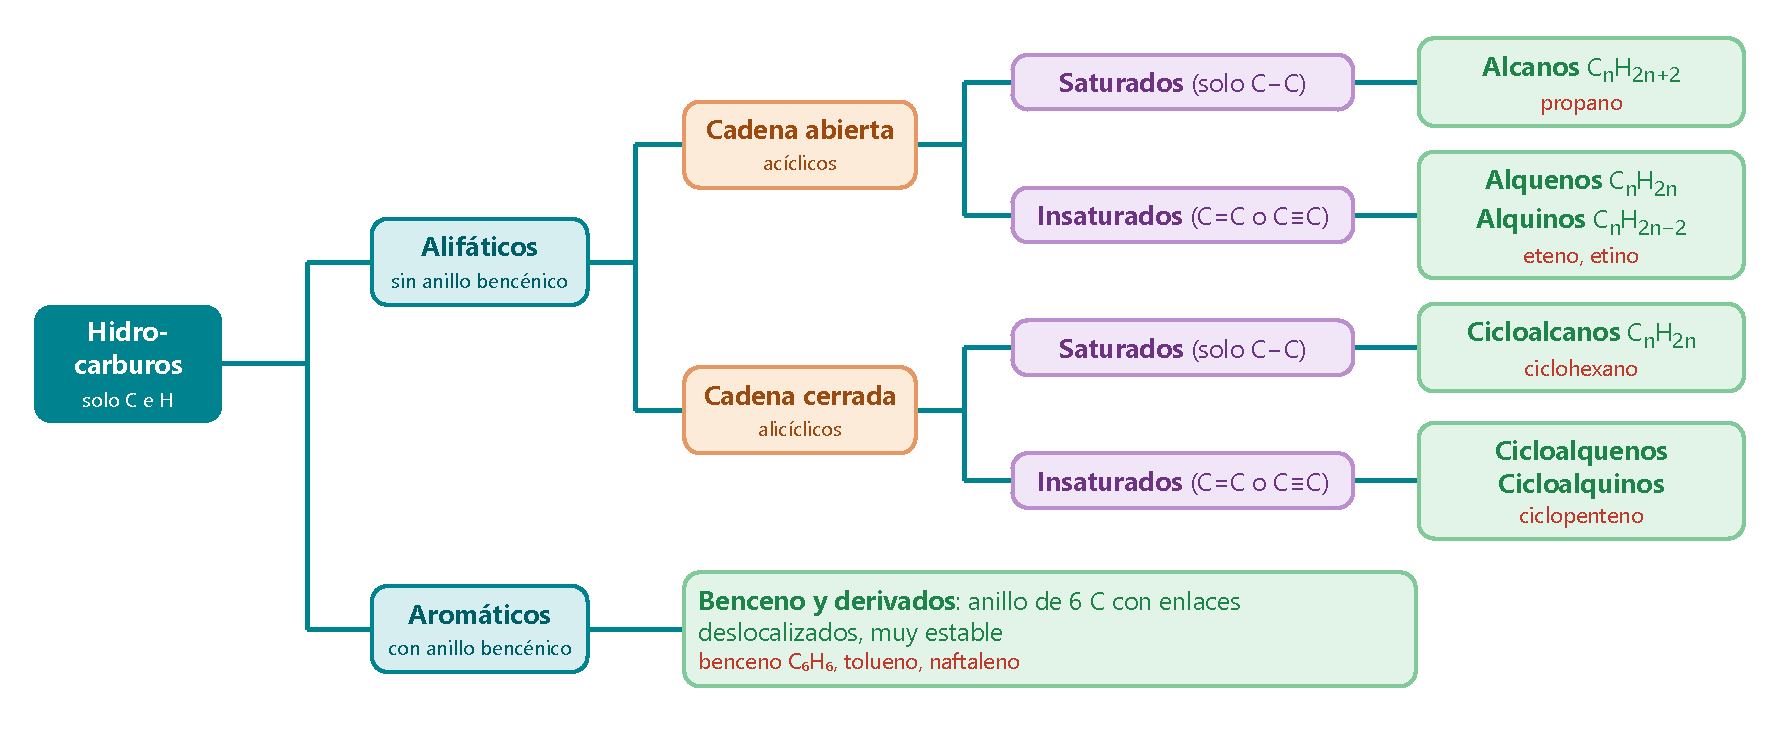
\includegraphics[width=\textwidth]{images/UD7/clasificacion_hidrocarburos}
    \caption{Clasificación de los hidrocarburos.}
    \label{fig:ud7-clasificacion}
\end{figure}

\subsection{Alcanos}

Los \textbf{alcanos} son hidrocarburos de cadena abierta con todos los enlaces \ch{C-C} sencillos. Su fórmula general es
\(\ch{C_nH_{2n+2}}\).

\paragraph{Alcanos de cadena lineal.} Se nombran con el prefijo del número de carbonos y la terminación \textbf{-ano}: \ch{CH4},
metano; \ch{CH3-CH2-CH2-CH3}, butano; \ch{CH3-(CH2)5-CH3}, heptano.

\paragraph{Radicales alquilo.} Son alcanos que han perdido un hidrógeno de un extremo. Se nombran cambiando -ano por \textbf{-ilo}
(o \textbf{-il} cuando se nombran como sustituyentes): \ch{CH3-}, metilo; \ch{CH3-CH2-}, etilo; \ch{CH3-CH2-CH2-}, propilo;
\ch{CH3-(CH2)3-}, butilo.

\paragraph{Alcanos ramificados.} Las ramificaciones son radicales alquilo unidos a la cadena principal. Para nombrarlos:
\begin{enumerate}
    \item Elige como cadena principal la \textbf{más larga}. Si hay varias igual de largas, la que tenga \textbf{más
    ramificaciones}.
    \item \textbf{Numera} la cadena desde el extremo que dé los \textbf{localizadores más bajos} a las ramificaciones (en el primer
    punto de diferencia). Si sigue habiendo empate, se da el localizador más bajo a la ramificación que se cita antes por orden
    alfabético.
    \item Nombra los radicales por \textbf{orden alfabético} con su localizador delante. Si hay varios iguales, se agrupan con
    di-, tri-\ldots\ y se escriben todos los localizadores, aunque se repitan: 3,3-dietil.
    \item Termina con el nombre de la cadena principal.
\end{enumerate}

\begin{example}
    \textbf{Nombrar un alcano ramificado.} Nombra el compuesto
    \[ \chemfig{CH_3-CH(-[6]CH_3)-CH(-[6]CH_2-[0]CH_3)-CH_2-CH_2-CH_3} \]

    \textbf{Solución.} Hay dos cadenas de 6 carbonos: la horizontal y la que entra por el etilo. La horizontal tiene dos
    ramificaciones (metilo y etilo); la otra, solo una (un radical de tres carbonos). Elegimos la horizontal. Numerando desde la
    izquierda, los localizadores son \{2, 3\}; desde la derecha, \{4, 5\}: numeramos desde la izquierda. Por orden alfabético
    (e antes que m): \textbf{3-etil-2-metilhexano}.
\end{example}

\begin{example}
    \textbf{Formular un alcano ramificado.} Formula el 5-etil-2,3,3-trimetilheptano.

    \textbf{Solución.} Cadena de 7 carbonos; metilos en C2 y dos en C3; etilo en C5. Completamos con hidrógenos:
    \[ \chemfig{CH_3-CH(-[6]CH_3)-C(-[2]CH_3)(-[6]CH_3)-CH_2-CH(-[6]CH_2-[0]CH_3)-CH_2-CH_3} \]
    La fórmula molecular es \ch{C12H26}, que cumple \(\ch{C_nH_{2n+2}}\).
\end{example}

\paragraph{Radicales complejos.} Los radicales ramificados se nombran como si fueran compuestos, numerando desde el carbono unido
a la cadena principal, y su nombre se escribe entre paréntesis: \ch{CH3-CH(CH3)-CH2-}, (2-metilpropil). La IUPAC admite nombres
tradicionales para los más sencillos:

\begin{table}[H]
    \centering
    \caption{Radicales ramificados con nombre tradicional}
    \vspace{-5pt}
    \begin{tabular}{@{}lll@{}}
        \toprule
        \textbf{Radical} & \textbf{Nombre tradicional} & \textbf{Nombre sistemático} \\
        \midrule
        \chemfig{CH_3-CH(-[6]CH_3)-} & isopropil & (1-metiletil) \\[3pt]
        \chemfig{CH_3-CH(-[6]CH_3)-CH_2-} & isobutil & (2-metilpropil) \\[3pt]
        \chemfig{CH_3-CH_2-CH(-[6]CH_3)-} & \emph{sec}-butil & (1-metilpropil) \\[3pt]
        \chemfig{CH_3-C(-[2]CH_3)(-[6]CH_3)-} & \emph{terc}-butil & (1,1-dimetiletil) \\[3pt]
        \chemfig{CH_3-C(-[2]CH_3)(-[6]CH_3)-CH_2-} & neopentil & (2,2-dimetilpropil) \\
        \bottomrule
    \end{tabular}
    \label{tab:ud7-radicales}
\end{table}

Al ordenar alfabéticamente, iso- y neo- sí cuentan (isopropil va por la i), pero \emph{sec}- y \emph{terc}- no (\emph{terc}-butil va
por la b).

\paragraph{Propiedades y aplicaciones.}
\begin{itemize}
    \item Son \textbf{apolares}: sus moléculas se atraen solo por fuerzas de dispersión, por lo que sus puntos de fusión y
    ebullición son \textbf{bajos} y aumentan con el número de carbonos (figura~\ref{fig:ud7-ebullicion}). A temperatura ambiente
    son gases hasta 4 carbonos, líquidos hasta unos 17 y sólidos a partir de ahí (parafinas). Las ramificaciones hacen la molécula
    más compacta y \textbf{bajan} el punto de ebullición.
    \item Son \textbf{insolubles en agua} y solubles en disolventes apolares; su densidad es menor que la del agua.
    \item Son \textbf{poco reactivos} (de ahí el nombre de \emph{parafinas}, «poca afinidad»). Sus reacciones más importantes son la
    \textbf{combustión} y el \textbf{craqueo}, en el que los alcanos grandes se rompen con calor en otros más pequeños.
    \item Se obtienen del \textbf{petróleo} y del \textbf{gas natural} y se usan sobre todo como \textbf{combustibles}.
\end{itemize}

\begin{figure}[H]
    \centering
    \begin{tikzpicture}
        \begin{axis}[grafica, width=0.62\linewidth, height=5.5cm,
            xlabel={Número de carbonos}, ylabel={\(T_\text{eb}\) (\unit{\degreeCelsius})},
            xmin=0, xmax=11, ymin=-200, ymax=200, xtick={1,...,10}, ytick={-200,-100,...,200}]
            \addplot[thick, mark=*, color=ocre] coordinates {(1,-162) (2,-89) (3,-42) (4,-0.5) (5,36) (6,69) (7,98) (8,126) (9,151) (10,174)};
            \addplot[dashed, gray] coordinates {(0,25) (11,25)};
            \node[font=\scriptsize, gray, anchor=south west] at (axis cs:0.2,25) {\qty{25}{\degreeCelsius}};
        \end{axis}
    \end{tikzpicture}
    \caption{Temperatura de ebullición de los alcanos lineales: por debajo de la línea de \qty{25}{\degreeCelsius}, gases.}
    \label{fig:ud7-ebullicion}
\end{figure}

\begin{exercise}
    Formula: a) hexano; b) 2,3-dimetilpentano; c) 4-etil-3,3-dimetilheptano; d) 5-isopropil-3-metilnonano; e)
    4-\emph{terc}-butiloctano.
    \begin{solu}
        a) \textcolor{red}{\ch{CH3-(CH2)4-CH3}}. b) \textcolor{red}{\chemfig{CH_3-CH(-[6]CH_3)-CH(-[6]CH_3)-CH_2-CH_3}}.
        c) \textcolor{red}{\chemfig{CH_3-CH_2-C(-[2]CH_3)(-[6]CH_3)-CH(-[6]CH_2-[0]CH_3)-CH_2-CH_2-CH_3}}.
        d) \textcolor{red}{\chemfig{CH_3-CH_2-CH(-[6]CH_3)-CH_2-CH(-[6]CH(-[0]CH_3)-[6]CH_3)-(CH_2)_3-CH_3}}.
        e) \textcolor{red}{\chemfig{CH_3-CH_2-CH_2-CH(-[6]C(-[0]CH_3)(-[4]H_3C)-[6]CH_3)-(CH_2)_3-CH_3}}.
    \end{solu}
\end{exercise}

\begin{exercise}
    Nombra: a) \ch{CH3-(CH2)6-CH3};
    \begin{gather*}
        \text{b)}\ \chemfig{CH_3-C(-[2]CH_3)(-[6]CH_3)-CH(-[6]CH_3)-CH_3} \qquad
        \text{c)}\ \chemfig{CH_3-CH(-[6]CH_3)-CH_2-CH(-[6]CH_2-[0]CH_3)-CH_2-CH_3} \\
        \text{d)}\ \chemfig{CH_3-CH_2-CH(-[6]CH_3)-CH(-[6]CH_3)-CH_2-CH_2-CH_3} \qquad
        \text{e)}\ \chemfig{CH_3-CH(-[6]CH_3)-CH(-[2]CH_2-[0]CH_3)-CH(-[6]CH_3)-CH_3}
    \end{gather*}
    \begin{solu}
        a) \textcolor{red}{Octano}. b) \textcolor{red}{2,2,3-trimetilbutano}. c) \textcolor{blue}{Cadena de 6 C; localizadores
        \{2, 4\} frente a \{3, 5\}:} \textcolor{red}{4-etil-2-metilhexano}. d) \textcolor{red}{3,4-dimetilheptano}.
        e) \textcolor{blue}{Todas las cadenas posibles tienen 5 C; la horizontal tiene tres ramificaciones:}
        \textcolor{red}{3-etil-2,4-dimetilpentano}.
    \end{solu}
\end{exercise}

\begin{exercise}
    Ordena de menor a mayor punto de ebullición y justifica: hexano, propano, decano y 2,2-dimetilbutano.
    \begin{solu}
        \textcolor{red}{Propano \(<\) 2,2-dimetilbutano \(<\) hexano \(<\) decano}. Las fuerzas de dispersión crecen con el tamaño de
        la molécula. El hexano y el 2,2-dimetilbutano tienen la misma masa (\ch{C6H14}), pero la forma compacta del segundo reduce la
        superficie de contacto entre moléculas (hierven a 69 y \qty{50}{\degreeCelsius}).
    \end{solu}
\end{exercise}

\begin{exercise}
    a) Escribe y ajusta la combustión del octano, \ch{C8H18}. b) ¿Qué masa de \ch{CO2} se emite al quemar \qty{1}{\litre} de
    gasolina, suponiendo que es octano puro de densidad \qty{0.70}{\kilo\gram\per\litre}?
    \begin{solu}
        a) \textcolor{red}{\ch{2 C8H18 + 25 O2 -> 16 CO2 + 18 H2O}}. b) \textcolor{blue}{\(n(\ch{C8H18}) = 700/114 = \qty{6.14}{\mol}\);
        \(n(\ch{CO2}) = 8 \cdot 6{,}14 = \qty{49.1}{\mol}\).} \(m = 49{,}1 \cdot 44 = \textcolor{red}{\qty{2.16}{\kilo\gram}}\).
    \end{solu}
\end{exercise}

\subsection{Alquenos y alquinos}

Los \textbf{alquenos} tienen algún enlace doble \ch{C=C}, y los \textbf{alquinos}, algún enlace triple \ch{C+C}. Con una sola
insaturación, sus fórmulas generales son \(\ch{C_nH_{2n}}\) y \(\ch{C_nH_{2n-2}}\).

\paragraph{Cadena lineal con una insaturación.} Se cambia la terminación -ano por \textbf{-eno} (doble) o \textbf{-ino} (triple):
\ch{CH2=CH2}, eteno o etileno; \ch{CH+CH}, etino o acetileno. A partir de 4 carbonos hay que indicar la posición del enlace
múltiple: se numera desde el extremo \textbf{más próximo} a él y se escribe el \textbf{menor} de los dos localizadores delante de la
terminación: \ch{CH2=CH-CH2-CH3}, but-1-eno; \ch{CH3-C+C-CH2-CH3}, pent-2-ino.

\paragraph{Varias insaturaciones.} Se usan \textbf{-dieno}, \textbf{-trieno}, \textbf{-diino}\ldots, y se añade una «a» a la raíz
cuando lo pide la pronunciación: buta-1,3-dieno, hexa-1,3,5-trieno. Si hay dobles y triples enlaces, se nombran primero los
dobles (\textbf{-en-}) y luego los triples (\textbf{-ino}), y se numera para que el \textbf{conjunto} de los localizadores de los
enlaces múltiples sea el más bajo; si hay empate, los dobles enlaces reciben los más bajos:
\[ \underset{\text{pent-1-en-4-ino}}{\ch{CH2=CH-CH2-C+CH}} \qquad\qquad
   \underset{\text{hexa-1,3-dien-5-ino}}{\ch{CH+C-CH=CH-CH=CH2}} \]

\paragraph{Radicales.} Los radicales con un doble o triple enlace se numeran desde el carbono por el que se unen: \ch{CH2=CH-},
etenil (vinil); \ch{CH2=CH-CH2-}, prop-2-enil (alil); \ch{CH+C-}, etinil.

\paragraph{Alquenos y alquinos ramificados.} Las ramificaciones se nombran delante, en orden alfabético. Según las recomendaciones
actuales de la IUPAC, la cadena principal se elige así (si hay empate en un criterio, se pasa al siguiente):
\begin{enumerate}
    \item la de mayor número de carbonos;
    \item la de mayor número de enlaces múltiples;
    \item la de mayor número de enlaces dobles.
\end{enumerate}
Después, se numera para dar los localizadores más bajos a los enlaces múltiples en conjunto, luego a los dobles y, por último, a
las ramificaciones.

\begin{example}
    \textbf{Nombrar alquenos y alquinos.} Nombra:
    \begin{gather*}
        \text{a)}\ \chemfig{CH_3-CH=C(-[6]CH_3)-CH_2-CH_3} \qquad \text{b)}\ \chemfig{CH_2=CH-CH(-[6]CH_2-[0]CH_3)-C~CH} \\
        \text{c)}\ \chemfig{CH_3-C~C-CH_2-CH(-[6]CH_3)-CH_3}
    \end{gather*}

    \textbf{Solución.} a) Cadena de 5 C; numerando desde la izquierda el doble enlace está en el C2. Metilo en C3:
    \textbf{3-metilpent-2-eno}. b) Todas las cadenas posibles tienen 5 C, pero la horizontal contiene los dos enlaces múltiples. Los
    localizadores son \{1, 4\} por ambos lados; desempata el doble enlace, que recibe el 1: \textbf{3-etilpent-1-en-4-ino}. c)
    Cadena de 6 C; el triple enlace está más cerca de la izquierda (C2): \textbf{5-metilhex-2-ino}.
\end{example}

\paragraph{Propiedades y aplicaciones.} Como los alcanos, son \textbf{poco polares}, con puntos de fusión y ebullición bajos,
\textbf{insolubles en agua} y menos densos que ella. Los alquinos tienen puntos de ebullición algo mayores que los alquenos, y estos
que los alcanos del mismo número de carbonos. Sus enlaces múltiples los hacen \textbf{más reactivos}: además de arder, dan
reacciones de \textbf{adición} (por ejemplo, de \ch{H2} para dar alcanos o de \ch{HCl} para dar derivados halogenados) y de
\textbf{polimerización}, en la que muchas moléculas se unen formando una cadena gigante, como el polietileno (PE) o el policloruro de
vinilo (PVC). El \textbf{eteno} es la sustancia que más fabrica la industria química, y las plantas lo producen como
\textbf{hormona de la maduración} de los frutos. El \textbf{etino} se quema en los sopletes de soldadura.

\begin{exercise}
    Formula: a) but-1-eno; b) pent-2-ino; c) 2-metilbut-2-eno; d) hexa-1,4-dieno; e) 3-metilbut-1-ino; f) hex-1-en-5-ino;
    g) 4-etil-2-metilhexa-1,3-dieno; h) penta-1,3-diino.
    \begin{solu}
        a) \textcolor{red}{\ch{CH2=CH-CH2-CH3}}; b) \textcolor{red}{\ch{CH3-C+C-CH2-CH3}};
        c) \textcolor{red}{\chemfig{CH_3-C(-[6]CH_3)=CH-CH_3}}; d) \textcolor{red}{\ch{CH2=CH-CH2-CH=CH-CH3}};
        e) \textcolor{red}{\chemfig{CH~C-CH(-[6]CH_3)-CH_3}}; f) \textcolor{red}{\ch{CH2=CH-CH2-CH2-C+CH}};
        g) \textcolor{red}{\chemfig{CH_2=C(-[6]CH_3)-CH=C(-[6]CH_2-[0]CH_3)-CH_2-CH_3}}; h) \textcolor{red}{\ch{CH+C-C+C-CH3}}.
    \end{solu}
\end{exercise}

\begin{exercise}
    Nombra: a) \ch{CH3-CH=CH-CH2-CH3}; b) \ch{CH2=CH-CH=CH-CH3}; d) \ch{CH+C-CH=CH-CH=CH2};
    e) \ch{CH3-CH2-C+C-CH2-CH2-CH3};
    \[ \text{c)}\ \chemfig{CH_2=C(-[6]CH_3)-C(-[6]CH_3)=CH_2} \qquad\qquad \text{f)}\ \chemfig{CH_3-CH(-[6]CH_3)-CH=CH-C~CH} \]
    \begin{solu}
        a) \textcolor{red}{Pent-2-eno}; b) \textcolor{red}{penta-1,3-dieno}; c) \textcolor{red}{2,3-dimetilbuta-1,3-dieno};
        d) \textcolor{red}{hexa-1,3-dien-5-ino}; e) \textcolor{red}{hept-3-ino}; f) \textcolor{blue}{numerando desde la derecha,
        los enlaces múltiples tienen \{1, 3\} (frente a \{3, 5\}):} \textcolor{red}{5-metilhex-3-en-1-ino}.
    \end{solu}
\end{exercise}

\begin{exercise}
    a) Ajusta la combustión del etino. b) ¿Qué volumen de oxígeno, medido en condiciones normales, se necesita para quemar
    \qty{52}{\gram} de etino?
    \begin{solu}
        a) \textcolor{red}{\ch{2 C2H2 + 5 O2 -> 4 CO2 + 2 H2O}}. b) \textcolor{blue}{\(n(\ch{C2H2}) = 52/26 = \qty{2.0}{\mol}\);
        \(n(\ch{O2}) = 2{,}0 \cdot 5/2 = \qty{5.0}{\mol}\).} \(V = 5{,}0 \cdot 22{,}4 = \textcolor{red}{\qty{112}{\litre}}\).
    \end{solu}
\end{exercise}

\subsection{Hidrocarburos cíclicos}

Su cadena principal es \textbf{cerrada}. Los \textbf{alicíclicos} se nombran como los de cadena abierta anteponiendo el prefijo
\textbf{ciclo-}: \textbf{cicloalcanos} si solo tienen enlaces sencillos (fórmula general \(\ch{C_nH_{2n}}\)) y
\textbf{cicloalquenos} o \textbf{cicloalquinos} si tienen insaturaciones. Se suelen representar en esqueleto, como polígonos:
\[ \underset{\text{ciclopropano}}{\chemfig{*3(---)}} \qquad \underset{\text{ciclobutano}}{\chemfig{*4(----)}} \qquad
   \underset{\text{ciclopentano}}{\chemfig{*5(-----)}} \qquad \underset{\text{ciclohexano}}{\chemfig{*6(------)}} \]
Para las insaturaciones y los sustituyentes se siguen las mismas normas: los carbonos del doble enlace reciben los localizadores 1 y
2, y no hace falta escribir el localizador si no hay ambigüedad:
\[ \underset{\text{metilciclopropano}}{\chemfig{*3(--(-CH_3)-)}} \qquad
   \underset{\text{1,3-dimetilciclopentano}}{\chemfig{*5(-(-CH_3)--(-CH_3)--)}} \qquad
   \underset{\text{ciclohexeno}}{\chemfig{*6(=-----)}} \qquad
   \underset{\text{3-metilciclopenteno}}{\chemfig{*5(=-(-CH_3)---)}} \]

El \textbf{ciclohexano} es un líquido incoloro de olor dulce que se usa como disolvente y en la fabricación del nailon. Las
propiedades de los cicloalcanos se parecen a las de los alcanos, aunque su densidad y sus temperaturas de cambio de estado son algo
mayores.

\subsection{Hidrocarburos aromáticos}

En su origen se llamaron \emph{aromáticos} unos compuestos de olor agradable. Hoy se llama así a los compuestos que tienen un
anillo como el del \textbf{benceno}, \ch{C6H6}: seis carbonos en un hexágono plano con enlaces dobles y sencillos alternos. En
1865, \textbf{A. Kekulé} propuso que su estructura era intermedia entre dos formas; hoy sabemos que los seis enlaces \ch{C-C} son
iguales, intermedios entre sencillo y doble: los electrones de los dobles enlaces están \textbf{deslocalizados} por todo el anillo
(híbrido de \textbf{resonancia}). Por eso el benceno se dibuja también con un círculo:
\[ \chemfig{*6(=-=-=-)} \;\longleftrightarrow\; \chemfig{*6(-=-=-=)} \qquad \equiv \qquad \chemfig{**6(------)} \]

\paragraph{Nomenclatura.} El radical \ch{C6H5-} se llama \textbf{fenilo}.
\begin{itemize}
    \item Con \textbf{un sustituyente}, se antepone su nombre a «benceno»: metilbenceno (\textbf{tolueno}), etilbenceno,
    clorobenceno.
    \item Con \textbf{dos sustituyentes}, se indican sus posiciones con localizadores (1,2-, 1,3- o 1,4-) o con los prefijos
    \textbf{orto-} (\emph{o}-), \textbf{meta-} (\emph{m}-) y \textbf{para-} (\emph{p}-).
    \item Con \textbf{más de dos}, se numera el anillo para que los localizadores sean los más bajos, y los sustituyentes se citan por
    orden alfabético.
\end{itemize}
\[ \underset{\text{tolueno}}{\chemfig{*6(-=-=(-CH_3)-=)}} \qquad
   \underset{\text{1,2-dimetilbenceno (\emph{o}-)}}{\chemfig{*6(-=-=(-CH_3)-(-CH_3)=)}} \qquad
   \underset{\text{1-etil-3-metilbenceno (\emph{m}-)}}{\chemfig{*6(-=(-CH_3)-=(-CH_2-CH_3)-=)}} \qquad
   \underset{\text{1-cloro-4-metilbenceno (\emph{p}-)}}{\chemfig{*6(-=(-Cl)-=-(-CH_3)=)}} \]

\paragraph{Propiedades.} Son líquidos o sólidos a temperatura ambiente, apolares (insolubles en agua) y muy \textbf{estables}: no
dan fácilmente reacciones de adición, sino de sustitución, normalmente con catalizadores. Se obtienen del alquitrán de hulla y del
petróleo. El benceno es un disolvente y una materia prima muy importante, pero sus vapores son tóxicos y cancerígenos. El
2,4,6-trinitrotolueno (TNT) es un explosivo.

\begin{example}
    \textbf{Derivados del benceno.} a) Formula el 1,3,5-trimetilbenceno. b) Nombra el compuesto
    \[ \chemfig{*6(-=(-CH_2-CH_3)-=-(-CH_2-CH_3)=)} \]

    \textbf{Solución.} a) Tres metilos alternos en el anillo:
    \[ \chemfig{*6(-(-CH_3)=-(-CH_3)=-(-CH_3)=)} \]
    b) Dos etilos en posiciones 1 y 4: \textbf{1,4-dietilbenceno} o \emph{p}-dietilbenceno.
\end{example}

\begin{exercise}
    Formula o nombra: a) metilciclobutano; b) 1,2-dimetilciclohexano; c) ciclopenta-1,3-dieno; d) etilbenceno; e)
    1,3-dimetilbenceno; f) 1,4-diclorobenceno;
    \[ \text{g)}\ \chemfig{*6(-----(-CH_2-CH_3)-)} \qquad\qquad \text{h)}\ \chemfig{*6(-=-=(-CH(-[1]CH_3)-[7]CH_3)-=)} \]
    \begin{solu}
        a) \textcolor{red}{\chemfig{*4(---(-CH_3)-)}}; b) \textcolor{red}{\chemfig{*6(----(-CH_3)-(-CH_3)-)}};
        c) \textcolor{red}{\chemfig{*5(=-=--)}}; d) \textcolor{red}{\chemfig{*6(-=-=(-CH_2-CH_3)-=)}};
        e) \textcolor{red}{\chemfig{*6(-=(-CH_3)-=(-CH_3)-=)}} (\emph{m}-dimetilbenceno o \emph{m}-xileno);
        f) \textcolor{red}{\chemfig{*6(-=(-Cl)-=-(-Cl)=)}}; g) \textcolor{red}{etilciclohexano}; h) \textcolor{red}{isopropilbenceno}
        (cumeno).
    \end{solu}
\end{exercise}

\subsection{Derivados halogenados}

También llamados \textbf{haluros de alquilo}, resultan de sustituir átomos de hidrógeno de un hidrocarburo por átomos de halógeno
(F, Cl, Br, I), que se representan de forma genérica como \ch{-X}. Los halógenos se nombran como prefijos (\textbf{fluoro-,
cloro-, bromo-, yodo-}) en orden alfabético con el resto de los sustituyentes:
\[ \underset{\text{1-cloro-2-metilbutano}}{\chemfig{Cl-CH_2-CH(-[6]CH_3)-CH_2-CH_3}} \qquad
   \underset{\text{triclorometano (cloroformo)}}{\ch{CHCl3}} \qquad
   \underset{\text{4-bromopent-2-eno}}{\chemfig{CH_3-CH=CH-CH(-[6]Br)-CH_3}} \]

La polaridad del enlace \ch{C-X} hace que sus puntos de fusión y ebullición sean más altos que los del hidrocarburo del que
proceden, pero siguen siendo insolubles en agua. Se usan como disolventes, anestésicos, insecticidas (como el DDT, hoy prohibido por
su toxicidad) o para fabricar polímeros como el PVC o el teflón. Los \textbf{clorofluorocarbonos} (CFC), usados antes en
refrigeradores y aerosoles, destruyen la capa de ozono y están prohibidos desde el Protocolo de Montreal (1987).

\begin{exercise}
    Formula o nombra: a) 2-clorobutano; b) 1,2-dibromoetano; c) 1-bromo-3-cloropropano; d) bromobenceno; e) \ch{CH2=CHCl};
    f) \ch{CH3-CHCl-CHBr-CH3}; g) \ch{CF2=CF2}; h) \ch{CCl2F2}.
    \begin{solu}
        a) \textcolor{red}{\ch{CH3-CHCl-CH2-CH3}}; b) \textcolor{red}{\ch{CH2Br-CH2Br}}; c) \textcolor{red}{\ch{CH2Br-CH2-CH2Cl}};
        d) \textcolor{red}{\ch{C6H5Br}}; e) \textcolor{red}{cloroeteno} (cloruro de vinilo, el monómero del PVC);
        f) \textcolor{blue}{empate \{2, 3\}: el bromo, primero en el alfabeto, recibe el 2:} \textcolor{red}{2-bromo-3-clorobutano};
        g) \textcolor{red}{tetrafluoroeteno} (el monómero del teflón); h) \textcolor{red}{diclorodifluorometano} (un CFC).
    \end{solu}
\end{exercise}

%========================================================================================
\section{Compuestos oxigenados}\label{sec:ud7-oxigenados}
%========================================================================================

Pasamos a los compuestos con grupos funcionales: primero los que contienen \textbf{oxígeno} y después los que contienen
\textbf{nitrógeno}. Para elegir la cadena principal se aplican estos criterios por orden, pasando al siguiente solo si hay empate:
\begin{enumerate}
    \item Contiene el mayor número de grupos funcionales principales.
    \item Tiene el mayor número de carbonos.
    \item Tiene el mayor número de enlaces múltiples y, después, de dobles enlaces.
\end{enumerate}
Y se numera para dar los localizadores más bajos, por este orden: al grupo principal, a los enlaces múltiples (en conjunto, y
después a los dobles) y a los sustituyentes (en conjunto, y después al primero por orden alfabético).

\begin{figure}[H]
    \centering
    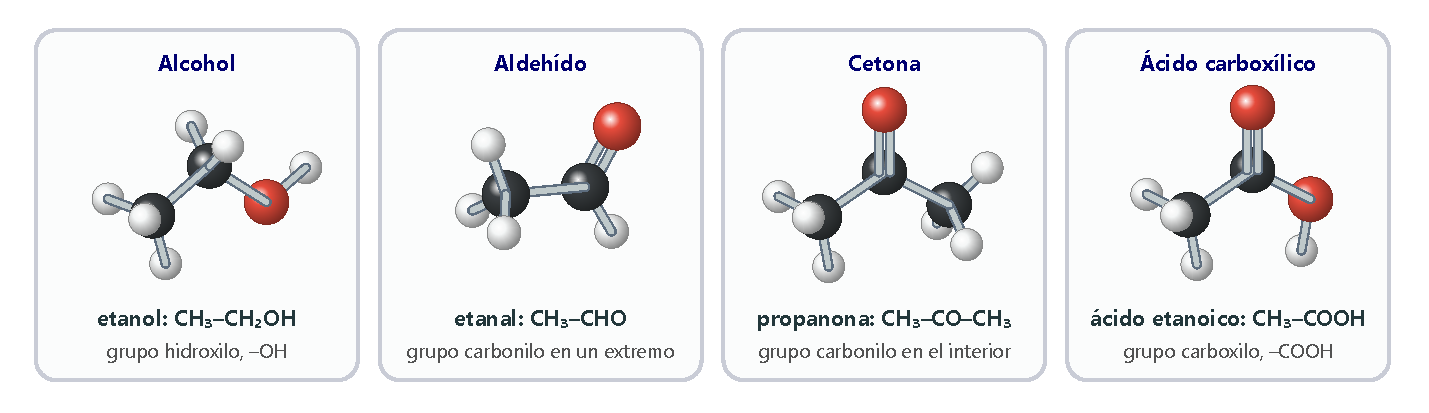
\includegraphics[width=\textwidth]{images/UD7/oxigenados}
    \caption{Modelos de bolas de los principales compuestos oxigenados de dos y tres carbonos.}
    \label{fig:ud7-oxigenados}
\end{figure}

\subsection{Alcoholes y fenoles}

Contienen el grupo \textbf{hidroxilo}, \ch{-OH}. En los \textbf{alcoholes} va unido a una cadena alifática (\ch{R-OH}), y en los
\textbf{fenoles}, a un anillo aromático (\ch{Ar-OH}). Los alcoholes son \textbf{primarios}, \textbf{secundarios} o
\textbf{terciarios} según el carbono que lleva el \ch{-OH}.

\paragraph{Nomenclatura.} Se añade el sufijo \textbf{-ol} al nombre del hidrocarburo, con el localizador del \ch{-OH} delante; con
varios grupos, \textbf{-diol}, \textbf{-triol}\ldots\ (polialcoholes, que conservan la «o» del hidrocarburo). Como sustituyente, el
\ch{-OH} se nombra \textbf{hidroxi-}.
\[ \underset{\text{etanol}}{\ch{CH3-CH2OH}} \qquad
   \underset{\text{3-metilbut-3-en-1-ol}}{\chemfig{CH_2=C(-[6]CH_3)-CH_2-CH_2OH}} \qquad
   \underset{\text{propano-1,2-diol}}{\ch{CH2OH-CHOH-CH3}} \]
Dos grupos \ch{-OH} no suelen estar en el mismo carbono, ni un \ch{-OH} en un carbono con doble enlace (esos compuestos son
inestables). En los fenoles se numera el anillo para que los \ch{-OH} tengan los localizadores más bajos:
\[ \underset{\text{fenol}}{\chemfig{*6(-=-=(-OH)-=)}} \qquad
   \underset{\text{benceno-1,3-diol}}{\chemfig{*6(-=(-OH)-=(-OH)-=)}} \qquad
   \underset{\text{4-metilfenol}}{\chemfig{*6(-=(-CH_3)-=-(-OH)=)}} \]

\paragraph{Propiedades y aplicaciones.} El grupo \ch{-OH} permite formar \textbf{enlaces de hidrógeno} entre moléculas
(figura~\ref{fig:ud7-hidrogeno}): por eso sus puntos de fusión y ebullición son mucho \textbf{más altos} que los de los
hidrocarburos de masa parecida, y los de menos carbonos son \textbf{solubles en agua}. La solubilidad disminuye al alargarse la
cadena, que es apolar. El \textbf{etanol} se obtiene por fermentación de azúcares y se usa como bebida, disolvente, desinfectante y
combustible (bioetanol); el \textbf{metanol} es muy tóxico; el \textbf{propan-2-ol} (alcohol isopropílico) limpia componentes
electrónicos, y la \textbf{glicerina} (propano-1,2,3-triol) se usa en cosmética.

\begin{figure}[H]
    \centering
    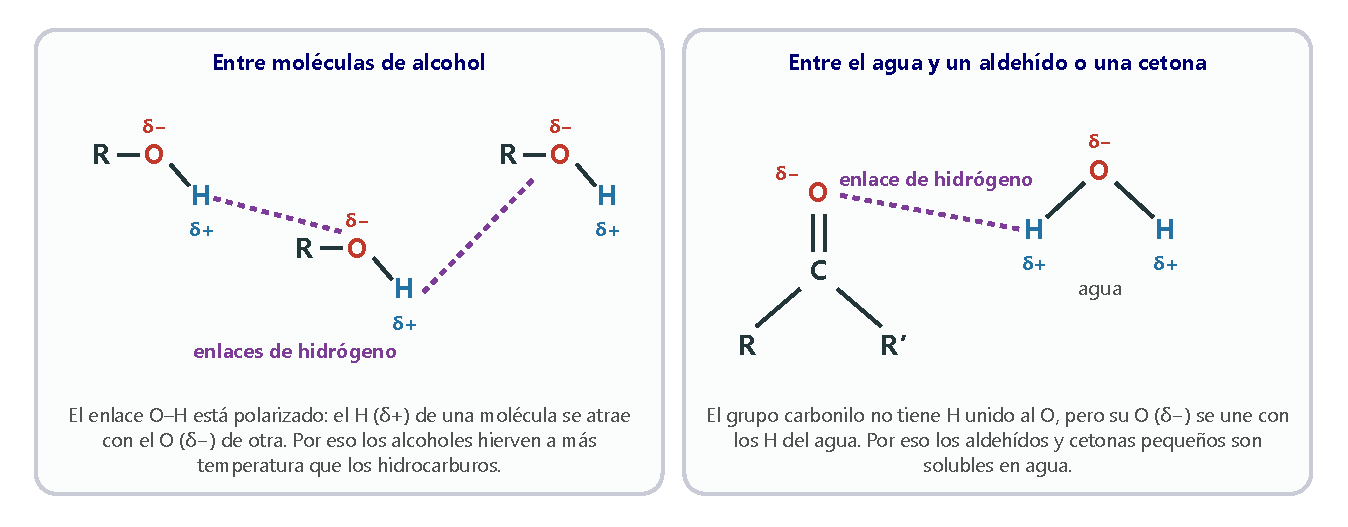
\includegraphics[width=0.95\textwidth]{images/UD7/enlace_hidrogeno}
    \caption{Enlaces de hidrógeno entre moléculas de alcohol y entre el agua y un compuesto con grupo carbonilo.}
    \label{fig:ud7-hidrogeno}
\end{figure}

\begin{exercise}
    Formula o nombra, e indica si los alcoholes son primarios, secundarios o terciarios: a) propan-2-ol; b) butano-1,3-diol; c)
    2-metilbutan-2-ol; d) but-3-en-1-ol; e) 3-metilfenol; f) \ch{CH3-CH2-CHOH-CH3}; g) \ch{CH2OH-CH2OH};
    h) \ch{CH2OH-CHOH-CH2OH}; i) \ch{CH3-CH=CH-CH2OH}.
    \begin{solu}
        a) \textcolor{red}{\ch{CH3-CHOH-CH3}, secundario}; b) \textcolor{red}{\ch{CH2OH-CH2-CHOH-CH3}, primario y secundario};
        c) \textcolor{red}{\chemfig{CH_3-C(-[2]OH)(-[6]CH_3)-CH_2-CH_3}, terciario}; d) \textcolor{red}{\ch{CH2=CH-CH2-CH2OH}, primario};
        e) \textcolor{red}{\chemfig{*6(-=(-CH_3)-=(-OH)-=)}}; f) \textcolor{red}{butan-2-ol, secundario};
        g) \textcolor{red}{etano-1,2-diol} (etilenglicol, anticongelante); h) \textcolor{red}{propano-1,2,3-triol} (glicerina);
        i) \textcolor{red}{but-2-en-1-ol, primario}.
    \end{solu}
\end{exercise}

\subsection{Éteres}

Su grupo funcional es un oxígeno unido a dos radicales: \ch{R-O-R'}. Se pueden nombrar de dos formas:
\begin{itemize}
    \item \textbf{Nombre de clase funcional}: los dos radicales en orden alfabético y la palabra \textbf{éter}:
    \ch{CH3-O-CH2-CH2-CH3}, metil propil éter.
    \item \textbf{Nomenclatura de sustitución} (la preferida por la IUPAC): el radical más sencillo con la terminación
    \textbf{-oxi} (\ch{CH3-O-}, metoxi; \ch{CH3-CH2-O-}, etoxi), seguido del nombre del hidrocarburo más complejo:
    \ch{CH3-O-CH2-CH2-CH3}, 1-metoxipropano.
\end{itemize}
Los éteres son poco reactivos y tienen puntos de ebullición más bajos que los alcoholes, porque no forman enlaces de hidrógeno entre
sus moléculas. Muchos son líquidos volátiles e inflamables que se usan como disolventes; el dietil éter fue uno de los primeros
anestésicos. Los \textbf{éteres corona}, cíclicos y con muchos oxígenos, atrapan cationes en su interior.

\begin{exercise}
    Formula o nombra de las dos formas: a) dietil éter; b) metoxibenceno; c) \ch{CH3-O-CH2-CH2-CH3}; d) \ch{CH3-CH2-O-CH=CH2};
    e) \chemfig{CH_3-CH_2-O-CH(-[6]CH_3)-CH_3}.
    \begin{solu}
        a) \textcolor{red}{\ch{CH3-CH2-O-CH2-CH3}, etoxietano}; b) \textcolor{red}{\ch{C6H5-O-CH3}, metil fenil éter} (anisol);
        c) \textcolor{red}{metil propil éter, 1-metoxipropano}; d) \textcolor{red}{etil vinil éter, etoxieteno};
        e) \textcolor{red}{etil isopropil éter, 2-etoxipropano}.
    \end{solu}
\end{exercise}

\subsection{Aldehídos y cetonas}

Ambos tienen el grupo \textbf{carbonilo}, \ch{C=O}.
\begin{itemize}
    \item En los \textbf{aldehídos} el carbonilo está en un \textbf{carbono terminal} (\ch{-CHO}). Se nombran con la terminación
    \textbf{-al}; no necesitan localizador, porque el \ch{-CHO} es siempre el C1: \ch{HCHO}, metanal (formaldehído);
    \ch{CH3-CH2-CHO}, propanal; \ch{OHC-CH2-CH2-CHO}, butanodial. Como sustituyente, \textbf{formil-} u \textbf{oxo-}.
    \item En las \textbf{cetonas} el carbonilo está en un \textbf{carbono intermedio} (\ch{-CO-}). Se nombran con la terminación
    \textbf{-ona} y el localizador más bajo posible: \ch{CH3-CO-CH3}, propanona (acetona); \ch{CH3-CO-CH2-CH2-CH3}, pentan-2-ona;
    \ch{CH3-CO-CH2-CO-CH2-CH3}, hexano-2,4-diona. Como sustituyente, \textbf{oxo-}. También se pueden nombrar citando los dos
    radicales y la palabra cetona: metil propil cetona.
\end{itemize}
En las fórmulas semidesarrolladas se escribe \ch{-OH} para los alcoholes y \ch{-CHO} para los aldehídos.

Por el grupo carbonilo, son compuestos \textbf{polares}: sus puntos de ebullición son más altos que los de los hidrocarburos, pero
menores que los de los alcoholes (no forman enlaces de hidrógeno entre sí, aunque sí con el agua, y por eso los pequeños son
solubles). Se obtienen oxidando alcoholes y se usan para fabricar resinas, plásticos, disolventes, pinturas y perfumes. La acetona
disuelve lacas y pinturas; el metanal (formol) conserva muestras biológicas.

\begin{remark}
    \textbf{Acetonemia.} Después de una fiebre o de pasar muchas horas sin comer, el organismo agota sus reservas de glucosa y
    obtiene energía de las grasas. En ese proceso se forma propanona, que se elimina por el aliento: por eso huele a acetona.
\end{remark}

\begin{exercise}
    Formula o nombra: a) etanal; b) butanona; c) 3-metilbutanal; d) pentan-3-ona; e) propenal; f) hexano-2,4-diona;
    g) \chemfig{CH_3-CH(-[6]CH_3)-CO-CH_3}; h) \ch{OHC-CH2-CH2-CHO}; i) \ch{C6H5-CHO}; j) \ch{CH3-CO-CH2-CH=CH2}.
    \begin{solu}
        a) \textcolor{red}{\ch{CH3-CHO}}; b) \textcolor{red}{\ch{CH3-CO-CH2-CH3}}; c) \textcolor{red}{\chemfig{CH_3-CH(-[6]CH_3)-CH_2-CHO}};
        d) \textcolor{red}{\ch{CH3-CH2-CO-CH2-CH3}}; e) \textcolor{red}{\ch{CH2=CH-CHO}}; f) \textcolor{red}{\ch{CH3-CO-CH2-CO-CH2-CH3}};
        g) \textcolor{red}{3-metilbutan-2-ona}; h) \textcolor{red}{butanodial}; i) \textcolor{red}{benzaldehído}
        (bencenocarbaldehído); j) \textcolor{blue}{la cetona tiene prioridad sobre el doble enlace:} \textcolor{red}{pent-4-en-2-ona}.
    \end{solu}
\end{exercise}

\subsection{Ácidos carboxílicos}

Su grupo funcional es el \textbf{carboxilo}, \ch{-COOH}, siempre en un extremo de la cadena. Se nombran con la palabra
\textbf{ácido} y la terminación \textbf{-oico}; el carbono del \ch{-COOH} es el C1:
\[ \underset{\text{ácido metanoico (fórmico)}}{\ch{HCOOH}} \qquad \underset{\text{ácido etanoico (acético)}}{\ch{CH3-COOH}}
   \qquad \underset{\text{ácido propanodioico}}{\ch{HOOC-CH2-COOH}} \qquad \underset{\text{ácido benzoico}}{\ch{C6H5-COOH}} \]

Son sustancias \textbf{polares} que forman enlaces de hidrógeno muy fuertes entre sí: sus puntos de ebullición son mayores que los
de los alcoholes. Los primeros de la serie son solubles en agua. Son \textbf{ácidos débiles} con muchas aplicaciones en la industria
\textbf{alimentaria} (vinagre, conservantes, acidulantes) y \textbf{farmacéutica}: el ácido acetilsalicílico es la aspirina.

\begin{exercise}
    Formula o nombra: a) ácido butanoico; b) ácido 2-metilpropanoico; c) ácido but-2-enoico; d) ácido etanodioico (oxálico); e)
    \chemfig{CH_3-CH_2-CH(-[6]CH_3)-COOH}; f) \ch{CH2=CH-COOH}; g) \ch{HOOC-CH2-CH2-COOH}.
    \begin{solu}
        a) \textcolor{red}{\ch{CH3-CH2-CH2-COOH}}; b) \textcolor{red}{\chemfig{CH_3-CH(-[6]CH_3)-COOH}};
        c) \textcolor{red}{\ch{CH3-CH=CH-COOH}}; d) \textcolor{red}{\ch{HOOC-COOH}}; e) \textcolor{red}{ácido 2-metilbutanoico};
        f) \textcolor{red}{ácido propenoico} (acrílico); g) \textcolor{red}{ácido butanodioico} (succínico).
    \end{solu}
\end{exercise}

\subsection{Ésteres y sales}

Los \textbf{ésteres} resultan de sustituir el H del grupo carboxilo por un radical: \ch{R-COO-R'}. Se forman al reaccionar un
ácido con un alcohol (\textbf{esterificación}):
\[ \ch{CH3-COOH + HO-CH2-CH3 <=> CH3-COO-CH2-CH3 + H2O} \]
Se nombran cambiando la terminación -oico del ácido por \textbf{-oato}, seguida de \textbf{de} y el nombre del radical acabado en
\textbf{-ilo}: \ch{CH3-COO-CH2-CH3}, etanoato de etilo (acetato de etilo); \ch{CH3-CH2-CH2-COO-CH3}, butanoato de metilo.

Los ésteres de baja masa molecular son líquidos volátiles de \textbf{olor agradable} a frutas o flores, que se usan en perfumes y
aromas alimentarios; los de masa alta son sólidos, como las ceras y las grasas.

Si el H del carboxilo se sustituye por un metal se obtienen \textbf{sales}, que se nombran como los ésteres con el nombre del
metal: \ch{CH3-COONa}, etanoato de sodio; \ch{CH3-CH2-COOK}, propanoato de potasio. Los \textbf{jabones} son sales de sodio o
potasio de ácidos de cadena larga.

\begin{exercise}
    Formula o nombra: a) etanoato de metilo; b) metanoato de etilo; c) propanoato de propilo; d) benzoato de metilo;
    e) butanoato de sodio; f) \ch{CH3-COO-CH2-CH2-CH3}; g) \ch{CH3-CH2-COO-CH3}; h) \ch{HCOOK}; i) \ch{CH3-COO-C6H5}.
    \begin{solu}
        a) \textcolor{red}{\ch{CH3-COO-CH3}}; b) \textcolor{red}{\ch{HCOO-CH2-CH3}}; c) \textcolor{red}{\ch{CH3-CH2-COO-CH2-CH2-CH3}};
        d) \textcolor{red}{\ch{C6H5-COO-CH3}}; e) \textcolor{red}{\ch{CH3-CH2-CH2-COONa}}; f) \textcolor{red}{etanoato de propilo}
        (aroma de pera); g) \textcolor{red}{propanoato de metilo}; h) \textcolor{red}{metanoato de potasio};
        i) \textcolor{red}{etanoato de fenilo}.
    \end{solu}
\end{exercise}

%========================================================================================
\section{Compuestos nitrogenados}\label{sec:ud7-nitrogenados}
%========================================================================================

\subsection{Aminas}

Derivan del \textbf{amoníaco}, \ch{NH3}, al sustituir uno, dos o tres hidrógenos por radicales: son aminas \textbf{primarias}
(\ch{R-NH2}), \textbf{secundarias} (\ch{R-NH-R'}) o \textbf{terciarias} (figura~\ref{fig:ud7-aminas}).
\begin{itemize}
    \item \textbf{Primarias}: se cambia la -o final del hidrocarburo por \textbf{-amina}: \ch{CH3-NH2}, metanamina;
    \ch{CH3-CH2-CH2-NH2}, propan-1-amina.
    \item \textbf{Secundarias y terciarias}: se toma como cadena principal el radical más complejo y los demás se nombran como
    sustituyentes precedidos de \textbf{N-}: \ch{CH3-NH-CH2-CH3}, N-metiletanamina; \ch{(CH3)2N-CH2-CH2-CH2-CH3},
    N,N-dimetilbutan-1-amina.
    \item Como sustituyente, el grupo \ch{-NH2} se llama \textbf{amino-}. La amina aromática más sencilla, \ch{C6H5-NH2}, es la
    \textbf{anilina} (fenilamina o bencenamina).
\end{itemize}

\begin{figure}[H]
    \centering
    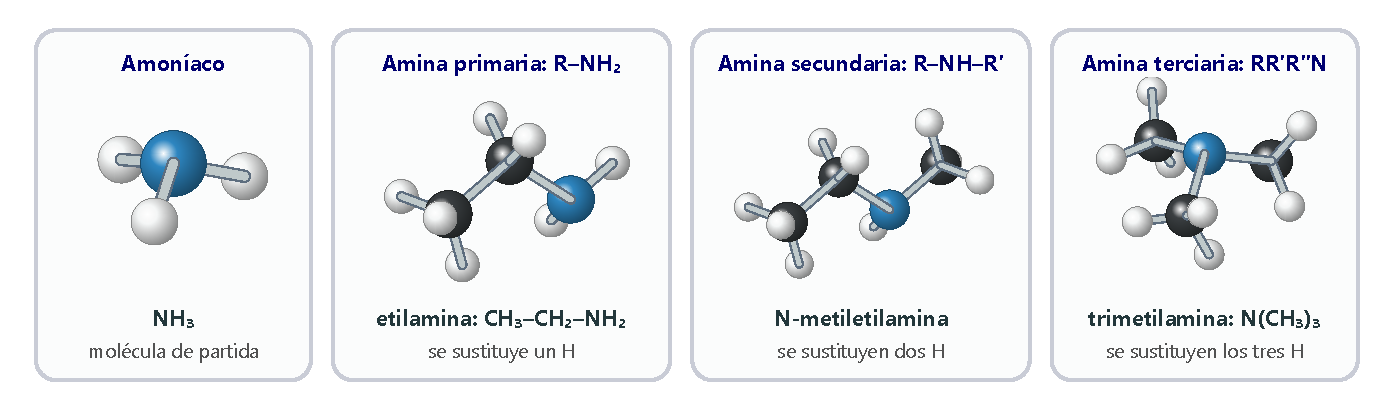
\includegraphics[width=\textwidth]{images/UD7/aminas}
    \caption{El amoníaco y las aminas primarias, secundarias y terciarias.}
    \label{fig:ud7-aminas}
\end{figure}

Por la polaridad del enlace \ch{N-H}, las aminas de baja masa molecular son solubles en agua. Son \textbf{bases}, con olor a
pescado podrido, que reaccionan fácilmente con los ácidos. Se usan para fabricar detergentes, colorantes y fármacos.

\subsection{Amidas}

Resultan de sustituir el \ch{-OH} de un ácido carboxílico por un grupo amino: \ch{R-CONH2}.
\begin{itemize}
    \item \textbf{Primarias}: se cambia la terminación -oico del ácido por \textbf{-amida}: \ch{CH3-CH2-CONH2}, propanamida.
    \item \textbf{Secundarias y terciarias}: se anteponen los radicales unidos al nitrógeno precedidos de \textbf{N-}:
    \ch{CH3-CO-NH-CH2-CH3}, N-etiletanamida; \ch{CH3-CO-N(CH3)-CH2-CH2-CH3}, N-metil-N-propiletanamida.
\end{itemize}
Las amidas son bases muy débiles y sustancias estables; salvo la metanamida, son \textbf{sólidas} a temperatura ambiente. Son muy
comunes en la naturaleza: las proteínas están formadas por aminoácidos unidos por enlaces de tipo amida (\textbf{enlace
peptídico}), y el \textbf{nailon} es una poliamida sintética.

\subsection{Nitrilos}

Tienen el grupo \ch{-C+N} en un extremo de la cadena. Se nombran con la terminación \textbf{-nitrilo}, contando el carbono del
grupo: \ch{CH3-C+N}, etanonitrilo (acetonitrilo); \ch{CH3-CH2-CH2-C+N}, butanonitrilo. Como sustituyente, \textbf{ciano-}. El
propenonitrilo (acrilonitrilo) es el monómero de fibras acrílicas.

\begin{example}
    \textbf{Compuestos nitrogenados.} a) Formula la N,N-dimetilpropanamida y la propan-2-amina. b) Nombra \ch{CH3-CH2-NH-CH2-CH3}
    y \ch{CH3-CH2-CH2-CH2-CONH2}.

    \textbf{Solución.} a) \ch{CH3-CH2-CO-N(CH3)2}: amida de tres carbonos con dos metilos en el N. \ch{CH3-CH(NH2)-CH3}: amina
    primaria con el \ch{-NH2} en el C2. b) Amina secundaria con dos etilos: \textbf{N-etiletanamina} (dietilamina). Amida primaria de
    5 carbonos: \textbf{pentanamida}.
\end{example}

\begin{exercise}
    Formula o nombra: a) etanamina; b) N-metilpropan-1-amina; c) N,N-dimetiletanamina; d) etanamida; e) N-metilbutanamida;
    f) fenilamina; g) \ch{H2N-CH2-CH2-NH2}; h) \ch{CH3-CO-N(CH3)2}; i) \ch{CH3-CH2-C+N}; j) \ch{CH3-CH2-N(CH3)-CH3}.
    \begin{solu}
        a) \textcolor{red}{\ch{CH3-CH2-NH2}}; b) \textcolor{red}{\ch{CH3-NH-CH2-CH2-CH3}}; c) \textcolor{red}{\ch{(CH3)2N-CH2-CH3}};
        d) \textcolor{red}{\ch{CH3-CONH2}}; e) \textcolor{red}{\ch{CH3-CH2-CH2-CO-NH-CH3}}; f) \textcolor{red}{\ch{C6H5-NH2}};
        g) \textcolor{red}{etano-1,2-diamina}; h) \textcolor{red}{N,N-dimetiletanamida}; i) \textcolor{red}{propanonitrilo};
        j) \textcolor{red}{N,N-dimetiletanamina}.
    \end{solu}
\end{exercise}

%========================================================================================
\section{Compuestos con varios grupos funcionales}\label{sec:ud7-varios}
%========================================================================================

Cuando hay más de un grupo funcional, se aplica la tabla~\ref{tab:ud7-prioridad}: el de mayor prioridad se nombra con su sufijo y
los demás, como prefijos, en orden alfabético con las ramificaciones y los halógenos.

\begin{example}
    \textbf{Nombrar un compuesto con varios grupos.} Nombra \chemfig{CH_3-CO-CH_2-CH(-[6]CH_3)-COOH}.

    \textbf{Solución.} 1) Grupos: \ch{-COOH} (ácido) y \ch{-CO-} (cetona). El ácido tiene prioridad: sufijo \emph{-oico}; la cetona
    será el prefijo \emph{oxo-}. 2) Cadena principal: 5 carbonos, numerados desde el \ch{-COOH} (C1). 3) Sustituyentes: metilo en
    C2 y oxo en C4. 4) Por orden alfabético (m antes que o): \textbf{ácido 2-metil-4-oxopentanoico}.
\end{example}

\begin{example}
    \textbf{Formular un compuesto con varios grupos.} Formula la 4-hidroxi-3-metilbutan-2-ona.

    \textbf{Solución.} El sufijo \emph{-ona} indica que la cetona es el grupo principal, en el C2 de una cadena de 4 carbonos. El
    \ch{-OH} (hidroxi) va en el C4 y un metilo en el C3:
    \[ \chemfig{CH_3-CO-CH(-[6]CH_3)-CH_2OH} \]
\end{example}

\begin{exercise}
    Formula o nombra: a) 2-hidroxipropanal; b) ácido 2-aminopropanoico (alanina); c) 4-oxopentanal; d) 3-hidroxibutan-2-ona;
    e) \ch{HOCH2-CH2-COOH}; f) \ch{CH3-CO-CH2-COOH}; g) \ch{H2N-CH2-CH2OH}; h) \ch{CH2=CH-CO-CH3}.
    \begin{solu}
        a) \textcolor{red}{\ch{CH3-CHOH-CHO}}; b) \textcolor{red}{\ch{CH3-CH(NH2)-COOH}}; c) \textcolor{red}{\ch{CH3-CO-CH2-CH2-CHO}};
        d) \textcolor{red}{\ch{CH3-CO-CHOH-CH3}}; e) \textcolor{red}{ácido 3-hidroxipropanoico}; f) \textcolor{red}{ácido
        3-oxobutanoico}; g) \textcolor{blue}{el alcohol tiene prioridad sobre la amina:} \textcolor{red}{2-aminoetanol};
        h) \textcolor{red}{but-3-en-2-ona}.
    \end{solu}
\end{exercise}

%========================================================================================
\section{Isomería}\label{sec:ud7-isomeria}
%========================================================================================

\begin{definition}[Isomería]
    Es la propiedad de los compuestos que tienen la \textbf{misma fórmula molecular} pero \textbf{distinta estructura}, y por tanto
    distintas propiedades. Estos compuestos se llaman \textbf{isómeros}.
\end{definition}

\subsection{Isomería estructural}

Los isómeros estructurales se diferencian en las \textbf{uniones} entre sus átomos:
\begin{itemize}
    \item \textbf{De cadena}: distinta cadena carbonada. \ch{C4H10}: butano, \ch{CH3-CH2-CH2-CH3}, y metilpropano,
    \chemfig{CH_3-CH(-[6]CH_3)-CH_3}.
    \item \textbf{De posición}: el mismo grupo funcional (o enlace múltiple) en distinta posición. \ch{C5H10O}: pentan-2-ona,
    \ch{CH3-CO-CH2-CH2-CH3}, y pentan-3-ona, \ch{CH3-CH2-CO-CH2-CH3}.
    \item \textbf{De función}: distinto grupo funcional. \ch{C4H10O}: butan-2-ol, \ch{CH3-CHOH-CH2-CH3}, y dietil éter,
    \ch{CH3-CH2-O-CH2-CH3}. Son pares típicos los alcoholes y los éteres, los aldehídos y las cetonas o los ácidos y los ésteres.
\end{itemize}

\subsection{Estereoisomería}

Los \textbf{estereoisómeros} tienen la misma fórmula molecular y la misma estructura (los mismos enlaces), pero sus átomos están
\textbf{distribuidos en el espacio} de distinta forma.

\paragraph{Isomería geométrica o cis-trans.} Aparece en compuestos con un doble enlace, porque este impide la rotación de los
carbonos que une. Si cada carbono del doble enlace tiene dos sustituyentes \textbf{distintos}, hay dos isómeros: \textbf{cis}, con
los grupos más voluminosos al mismo lado, y \textbf{trans}, en lados opuestos.
\[ \underset{\text{\emph{cis}-but-2-eno}}{\chemfig{C(-[3]H_3C)(-[5]H)=C(-[1]CH_3)(-[7]H)}} \qquad\qquad
   \underset{\text{\emph{trans}-but-2-eno}}{\chemfig{C(-[3]H_3C)(-[5]H)=C(-[1]H)(-[7]CH_3)}} \]
El but-1-eno, \ch{CH2=CH-CH2-CH3}, no tiene isómeros cis-trans: uno de sus carbonos tiene dos H iguales.

\paragraph{Isomería óptica.} La presentan las moléculas con un \textbf{carbono asimétrico} o \textbf{quiral}, unido a cuatro
sustituyentes distintos (se marca con un asterisco). Hay dos isómeros, los \textbf{enantiómeros}, que son imágenes especulares no
superponibles, como nuestras manos (figura~\ref{fig:ud7-enantiomeros}). Tienen casi todas las propiedades iguales, pero desvían
el plano de la luz polarizada en sentidos opuestos y actúan de forma distinta en los seres vivos: de muchos fármacos, como el
ibuprofeno, solo uno de los enantiómeros es activo.

\begin{figure}[H]
    \centering
    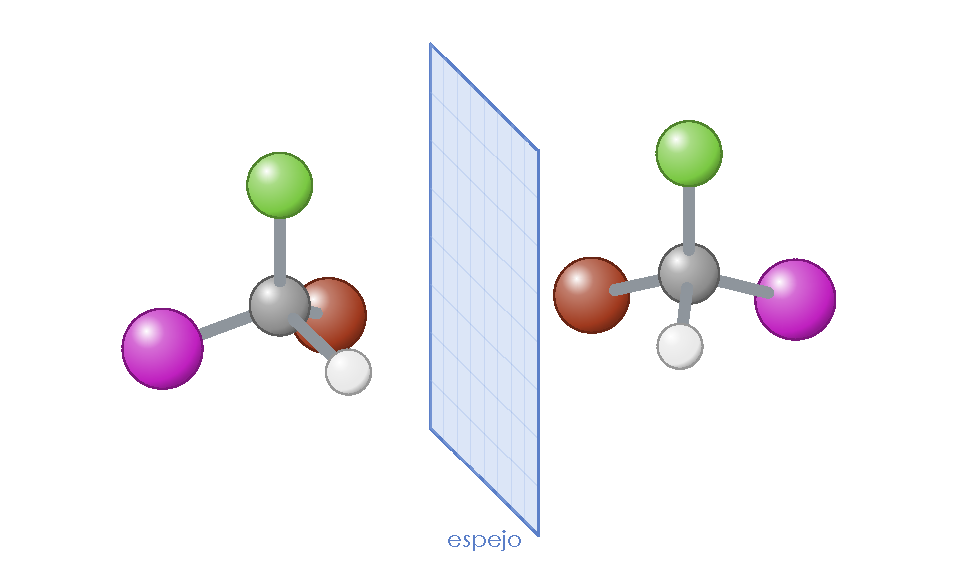
\includegraphics[width=0.55\textwidth]{images/UD7/enantiomeros}
    \caption{Dos enantiómeros: un carbono con cuatro sustituyentes distintos y su imagen en un espejo no se pueden superponer.}
    \label{fig:ud7-enantiomeros}
\end{figure}

\begin{example}
    \textbf{Buscar isómeros.} Escribe y nombra todos los isómeros de fórmula \ch{C3H8O}. ¿Qué tipo de isomería hay entre ellos?

    \textbf{Solución.} Con un \ch{-OH}: propan-1-ol, \ch{CH3-CH2-CH2OH}, y propan-2-ol, \ch{CH3-CHOH-CH3} (isómeros de
    \textbf{posición}). Con un \ch{-O-}: etil metil éter (metoxietano), \ch{CH3-O-CH2-CH3}, isómero de \textbf{función} de los dos
    alcoholes. Ninguno tiene carbono quiral ni doble enlace, así que no hay estereoisómeros.
\end{example}

\begin{exercise}
    Escribe y nombra los tres isómeros de cadena del \ch{C5H12} y los cinco hidrocarburos de cadena abierta de fórmula \ch{C6H14}.
    \begin{solu}
        \textcolor{red}{\ch{C5H12}: pentano, 2-metilbutano y 2,2-dimetilpropano.} \textcolor{red}{\ch{C6H14}: hexano,
        2-metilpentano, 3-metilpentano, 2,2-dimetilbutano y 2,3-dimetilbutano.}
    \end{solu}
\end{exercise}

\begin{exercise}
    Escribe dos isómeros de posición del \ch{C4H8} con un doble enlace y dos isómeros de función de fórmula \ch{C3H6O}.
    \begin{solu}
        \textcolor{red}{But-1-eno, \ch{CH2=CH-CH2-CH3}, y but-2-eno, \ch{CH3-CH=CH-CH3}.} \textcolor{red}{Propanal,
        \ch{CH3-CH2-CHO}, y propanona, \ch{CH3-CO-CH3}} (también el prop-2-en-1-ol, \ch{CH2=CH-CH2OH}).
    \end{solu}
\end{exercise}

\begin{exercise}
    ¿Cuáles presentan isomería cis-trans? Dibuja los dos isómeros cuando existan: a) propeno; b) pent-2-eno; c)
    2-metilbut-2-eno; d) 1,2-dicloroeteno.
    \begin{solu}
        a) \textcolor{red}{No} (el C1 tiene dos H). b) \textcolor{red}{Sí}: \chemfig{C(-[3]H_3C)(-[5]H)=C(-[1]CH_2-CH_3)(-[7]H)} (cis) y
        \chemfig{C(-[3]H_3C)(-[5]H)=C(-[1]H)(-[7]CH_2-CH_3)} (trans). c) \textcolor{red}{No} (el C2 tiene dos metilos). d)
        \textcolor{red}{Sí}: \chemfig{C(-[3]Cl)(-[5]H)=C(-[1]Cl)(-[7]H)} (cis) y \chemfig{C(-[3]Cl)(-[5]H)=C(-[1]H)(-[7]Cl)} (trans).
    \end{solu}
\end{exercise}

\begin{exercise}
    ¿Cuáles tienen un carbono quiral? Señálalo. a) Butan-2-ol; b) propan-2-ol; c) ácido 2-hidroxipropanoico (láctico); d)
    2-clorobutano; e) 3-metilpentano.
    \begin{solu}
        a) \textcolor{red}{Sí}, el C2 de \ch{CH3-CHOH-CH2-CH3}, unido a H, OH, \ch{CH3} y \ch{C2H5}. b) \textcolor{red}{No}: dos metilos iguales.
        c) \textcolor{red}{Sí}, el C2: H, OH, \ch{CH3} y \ch{COOH}. d) \textcolor{red}{Sí}, el C2. e) \textcolor{red}{No}: el C3
        tiene dos etilos iguales.
    \end{solu}
\end{exercise}

%========================================================================================
\section{Importancia de los compuestos del carbono}\label{sec:ud7-importancia}
%========================================================================================

\subsection{El petróleo y la industria petroquímica}

El \textbf{petróleo} es un líquido aceitoso, viscoso e inflamable, menos denso que el agua, formado por una mezcla de
\textbf{hidrocarburos} con pequeñas cantidades de compuestos de azufre, oxígeno y nitrógeno. Se formó durante millones de años a
partir de restos de plancton y algas enterrados a gran presión y temperatura, y se acumula en \textbf{yacimientos}. Una vez
extraído, el crudo se \textbf{refina}:
\begin{itemize}
    \item \textbf{Destilación fraccionada}: se calienta y se separa en fracciones según su temperatura de ebullición
    (figura~\ref{fig:ud7-destilacion}). Las de menos carbonos salen por arriba y las más pesadas, por abajo.
    \item \textbf{Transformaciones químicas}: el \textbf{craqueo} rompe los hidrocarburos pesados en otros más ligeros y en
    \textbf{olefinas} (alquenos como el eteno y el propeno), materia prima de los plásticos.
\end{itemize}

\begin{figure}[H]
    \centering
    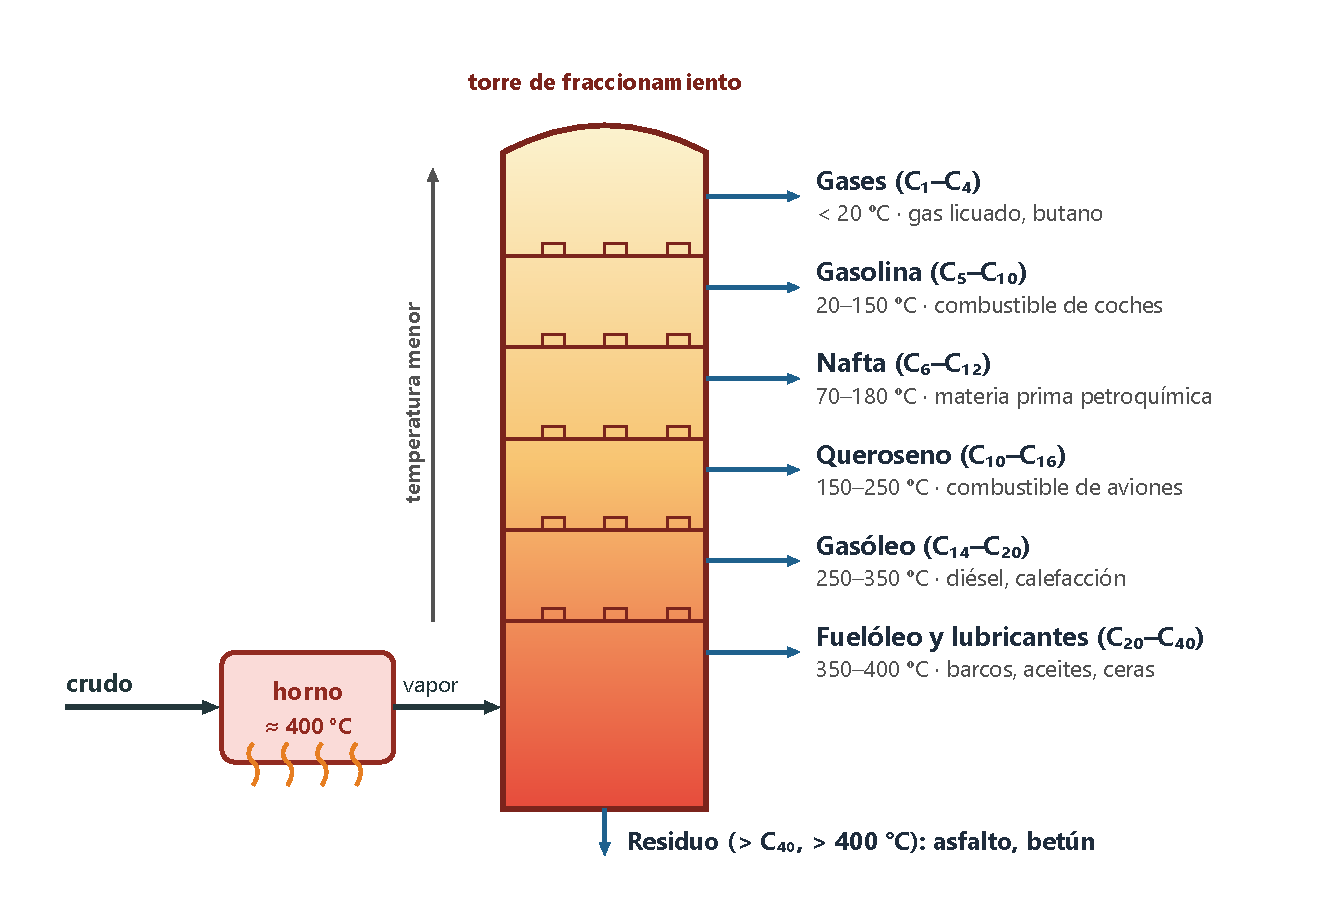
\includegraphics[width=0.85\textwidth]{images/UD7/torre_destilacion}
    \caption{Destilación fraccionada del petróleo.}
    \label{fig:ud7-destilacion}
\end{figure}

La \textbf{industria petroquímica} convierte estos productos en materias primas para fabricar plásticos, fibras sintéticas,
detergentes, anticongelantes, pinturas o fármacos: hasta un 60\,\% de los productos del mercado dependen de ella. Pero la
explotación del petróleo tiene un fuerte \textbf{impacto ambiental}: contaminación del suelo, el agua y el aire por derrames y
residuos (como la «marea negra» del \emph{Prestige} en Galicia, en 2002), deforestación para construir plataformas, carreteras y
oleoductos y, sobre todo, las emisiones de \ch{CO2} de su combustión, causa principal del cambio climático.

\subsection{Compuestos orgánicos de síntesis}

\begin{definition}[Síntesis orgánica]
    Es la construcción planificada de moléculas orgánicas complejas a partir de otras más sencillas mediante reacciones químicas.
\end{definition}

Desde la síntesis de la urea se han fabricado millones de moléculas: unas existen en la naturaleza y otras se han diseñado con un
fin concreto. Sus campos principales son los fármacos y los polímeros.

\paragraph{Síntesis de fármacos.} Fabricar un medicamento es un proceso largo en el que la primera etapa es obtener el
\textbf{principio activo}. Puede hacerse por \textbf{síntesis total}, a partir de sustancias sencillas y baratas, o por
\textbf{síntesis parcial}, partiendo de un compuesto extraído de la naturaleza. Para diseñar la ruta se usa el \textbf{análisis
retrosintético} de \textbf{E. J. Corey}: «desmontar» mentalmente la molécula objetivo en piezas cada vez más sencillas. El premio
Nobel de Química de 2022 fue para \textbf{B. Sharpless} y \textbf{M. Meldal}, por la \textbf{química clic}, que une bloques
moleculares de forma rápida y limpia, y para \textbf{C. Bertozzi}, que la llevó al interior de los organismos vivos.

\paragraph{Polímeros.} Los \textbf{polímeros} son macromoléculas formadas por la unión de muchas moléculas pequeñas, los
\textbf{monómeros}. Pueden ser \textbf{naturales} (celulosa, almidón, proteínas, caucho) o \textbf{sintéticos} (polietileno, PVC,
nailon, neopreno). La \textbf{polimerización} puede ser:
\begin{itemize}
    \item \textbf{por adición}: los monómeros, con un doble enlace, se unen sin perder átomos. Así se obtiene el
    \textbf{polietileno} a partir del eteno (figura~\ref{fig:ud7-polietileno}): \(n\,\ch{CH2=CH2} \rightarrow (\ch{-CH2-CH2-})_n\);
    \item \textbf{por condensación}: al unirse los monómeros se desprende una molécula pequeña, normalmente agua. Así se forman
    el nailon, el poliéster (PET) o las proteínas.
\end{itemize}
Los polímeros sintéticos son ligeros, fáciles de moldear, resistentes a la corrosión y aislantes. Se clasifican en
\textbf{plásticos}, \textbf{fibras} (nailon, poliéster) y \textbf{elastómeros} (neopreno, caucho sintético).

\begin{figure}[H]
    \centering
    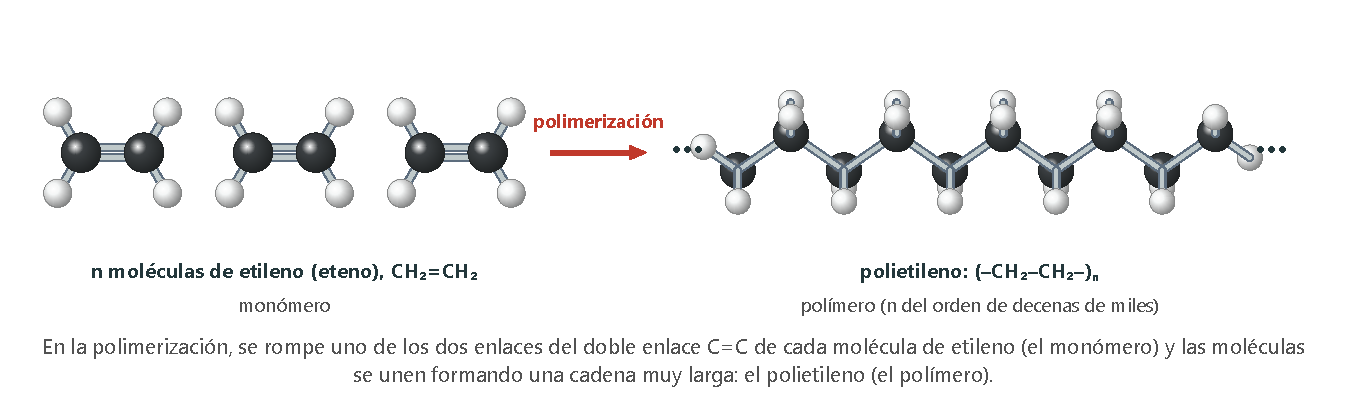
\includegraphics[width=0.9\textwidth]{images/UD7/polietileno}
    \caption{Polimerización por adición del eteno para dar polietileno.}
    \label{fig:ud7-polietileno}
\end{figure}

\subsection{Los compuestos orgánicos en los seres vivos}

Los seres vivos estamos formados en un 99\,\% por C, H, O, N, S y P, los \textbf{bioelementos} principales, que forman las
\textbf{biomoléculas}. La estructura de cada una determina su función:
\begin{itemize}
    \item \textbf{Glúcidos}: formados por C, H y O. Tienen función \textbf{energética} (la glucosa se «quema» en la respiración
    celular; el almidón y el glucógeno son reservas) y \textbf{estructural} (la celulosa de las paredes vegetales). Los
    monosacáridos, como la glucosa o la fructosa, se unen por condensación en disacáridos (la lactosa de la leche) y polisacáridos.
    \item \textbf{Lípidos}: insolubles en agua. Forman las membranas celulares y almacenan energía. Las \textbf{grasas saturadas}
    (mantequilla, embutidos) elevan el colesterol LDL y el riesgo cardiovascular; las \textbf{insaturadas} (aceite de oliva,
    pescado azul) ayudan a reducirlo.
    \item \textbf{Proteínas}: macromoléculas formadas por \textbf{aminoácidos}, compuestos con un grupo amino y un grupo ácido. Los
    aminoácidos se unen por condensación mediante el \textbf{enlace peptídico} (un enlace amida):
    \begin{gather*} \ch{H2N-CH2-COOH + H2N-CH(CH3)-COOH} \\ \ch{-> H2N-CH2-CO-NH-CH(CH3)-COOH + H2O} \end{gather*}
    Tienen funciones de transporte (hemoglobina), estructura (colágeno), hormonales (insulina), defensa (anticuerpos), movimiento
    (miosina) o catálisis (enzimas).
    \item \textbf{Ácidos nucleicos} (ADN y ARN), que almacenan y transmiten la información genética, y \textbf{vitaminas}, necesarias
    en pequeñas cantidades.
\end{itemize}

\begin{exercise}
    a) Escribe un fragmento de tres unidades del polipropileno, que se obtiene por adición del propeno. b) ¿Cuál es la masa molar de
    una cadena formada por \num{5000} monómeros?
    \begin{solu}
        a) \textcolor{red}{\ch{-CH2-CH(CH3)-CH2-CH(CH3)-CH2-CH(CH3)-}}: el doble enlace se abre y los metilos quedan como
        ramificaciones. b) \(M = 5000 \cdot 42 = \textcolor{red}{\qty{2.1e5}{\gram\per\mol}}\).
    \end{solu}
\end{exercise}

\begin{exercise}
    En el dipéptido de la ecuación anterior (glicina + alanina), señala el enlace peptídico, el grupo amino libre y el grupo
    carboxilo libre. ¿Qué tipo de reacción es? ¿Qué grupo funcional orgánico forma el enlace peptídico?
    \begin{solu}
        \textcolor{red}{El enlace peptídico es el \ch{-CO-NH-} central; el \ch{-NH2} libre está en el extremo de la glicina y el
        \ch{-COOH} libre, en el de la alanina.} Es una \textcolor{red}{condensación} (se desprende agua) y el enlace es una
        \textcolor{red}{amida}.
    \end{solu}
\end{exercise}

\begin{exercise}
    a) ¿Por qué el queroseno sale de la torre de destilación por encima del gasóleo? b) ¿Qué es el craqueo y para qué sirve? c) Cita
    tres impactos ambientales de la explotación del petróleo.
    \begin{solu}
        a) \textcolor{red}{Sus hidrocarburos son más pequeños (\ch{C10}--\ch{C16}) y tienen menor punto de ebullición}: condensan a
        menor temperatura, más arriba. b) \textcolor{red}{Romper con calor (y catalizadores) hidrocarburos pesados en otros más
        ligeros}, para obtener más gasolina y alquenos para la petroquímica. c) \textcolor{red}{Derrames que contaminan mares y
        costas, contaminación del aire y del suelo en las refinerías, deforestación y emisiones de \ch{CO2}} (cambio climático).
    \end{solu}
\end{exercise}

%========================================================================================
\section{Química en la vida: las mil caras del carbono}\label{sec:ud7-alotropos}
%========================================================================================

El carbono puro existe en varias formas, sus \textbf{alótropos}, con propiedades muy distintas. En el \textbf{diamante} cada átomo
está unido a otros cuatro en una red tridimensional rígida: es transparente, aislante y el material natural más duro. En el
\textbf{grafito} los átomos forman láminas de hexágonos apiladas, que se deslizan unas sobre otras: es blando, negro y conduce la
electricidad, porque cada carbono tiene un electrón deslocalizado.

En 1985, \textbf{H. Kroto}, \textbf{R. Curl} y \textbf{R. Smalley} descubrieron los \textbf{fullerenos}, moléculas huecas como el
\ch{C60}, con forma de balón de fútbol (premio Nobel de Química de 1996). En 1991, \textbf{S. Iijima} describió los
\textbf{nanotubos de carbono}, láminas de grafito enrolladas en cilindros, cien veces más resistentes que el acero y muy ligeros.
Y en 2004, \textbf{A. Geim} y \textbf{K. Novoselov} aislaron el \textbf{grafeno} pegando y despegando cinta adhesiva sobre un trozo
de grafito (premio Nobel de Física de 2010): una lámina de un solo átomo de grosor, flexible, transparente, más resistente que el
acero y mejor conductora que el cobre.

Estos materiales prometen pantallas flexibles, baterías de carga rápida, sensores, placas solares más eficientes, filtros para
potabilizar agua o transportar fármacos dentro del cuerpo. Todo, con el mismo elemento que forma la mina de un lápiz.

\begin{exercise}
    a) ¿Qué son los alótropos? b) ¿Por qué el grafito conduce la electricidad y el diamante no? c) El \ch{C60} tiene 60 átomos de
    carbono. ¿Cuál es su masa molar? ¿Cuántas moléculas hay en \qty{1}{\milli\gram}?
    \begin{solu}
        a) \textcolor{red}{Formas distintas de un mismo elemento}, con distinta estructura y propiedades. b) \textcolor{red}{En el
        grafito cada C se une solo a otros tres y le queda un electrón deslocalizado que puede moverse por la lámina}; en el diamante
        los cuatro electrones de valencia están en enlaces localizados. c) \(M = 60 \cdot 12 = \textcolor{red}{\qty{720}{\gram\per\mol}}\);
        \(N = \dfrac{\num{1e-3}}{720} \cdot \num{6.02e23} = \textcolor{red}{\num{8.4e17}}\) moléculas.
    \end{solu}
\end{exercise}

%========================================================================================
\section{Prácticas}\label{sec:ud7-practicas}
%========================================================================================

\subsection{Modelos moleculares con plastilina: isómeros}

\noindent\begin{minipage}[t]{0.48\textwidth}
    \textbf{Objetivo}
    \begin{itemize}
        \item Construir modelos de moléculas orgánicas para ver su forma en el espacio y comprobar que fórmulas moleculares iguales
        pueden dar estructuras distintas.
    \end{itemize}
\end{minipage}\hfill
\begin{minipage}[t]{0.48\textwidth}
    \textbf{Material}
    \begin{itemize}
        \item Plastilina de cuatro colores (negro para C, blanco para H, rojo para O y verde para Cl).
        \item Palillos de dientes y un transportador de ángulos.
    \end{itemize}
\end{minipage}

\textbf{Procedimiento}
\begin{enumerate}[label=\numberballgreen]
    \item Haz bolas de plastilina: las de C, algo más grandes que las de H.
    \item Construye el metano clavando cuatro palillos en una bola negra de forma que estén lo más separados posible. Mide el ángulo
    entre dos palillos.
    \item Construye el butano y el metilpropano (\ch{C4H10}). Gira los enlaces sencillos del butano: ¿cambia la molécula?
    \item Construye los dos isómeros del \ch{C2H6O}: el etanol y el dimetil éter.
    \item Para los dobles enlaces, une dos carbonos con dos palillos y construye el \emph{cis}- y el
    \emph{trans}-1,2-dicloroeteno. Intenta girar el doble enlace.
\end{enumerate}

\begin{exercise}
    a) ¿Qué ángulo aproximado has medido en el metano? ¿Cuál es el teórico? b) ¿Por qué girar los enlaces del butano no da un
    isómero nuevo y en el 1,2-dicloroeteno sí hay dos isómeros? c) Construye todos los isómeros del \ch{C3H6Cl2} y nómbralos.
    \begin{solu}
        a) \textcolor{red}{Unos \ang{110}; el teórico es \ang{109.5}}. b) \textcolor{red}{Los enlaces sencillos giran libremente:
        las distintas posiciones son la misma molécula. El doble enlace no puede girar}, así que los Cl quedan fijos al mismo lado o
        en lados opuestos. c) \textcolor{red}{1,1-dicloropropano, 1,2-dicloropropano, 1,3-dicloropropano y 2,2-dicloropropano}
        (el 1,2- tiene además un carbono quiral).
    \end{solu}
\end{exercise}

\subsection{Química en la cocina: fruta caramelizada}

\noindent\begin{minipage}[t]{0.48\textwidth}
    \textbf{Objetivo}
    \begin{itemize}
        \item Observar la \textbf{caramelización} del azúcar, una serie de reacciones de descomposición de la sacarosa por el calor, y
        preparar un tentempié de fruta.
    \end{itemize}
\end{minipage}\hfill
\begin{minipage}[t]{0.48\textwidth}
    \textbf{Material}
    \begin{itemize}
        \item \qty{150}{\gram} de fruta (manzana, pera, plátano\ldots), \qty{300}{\gram} de azúcar moreno o panela, una cucharada de
        miel y \qty{25}{\gram} de mantequilla.
        \item Sartén antiadherente, espátula, termómetro de cocina y papel de horno.
    \end{itemize}
\end{minipage}

\textbf{Procedimiento}
\begin{enumerate}[label=\numberballgreen]
    \item Lava la fruta, quítale las semillas y trocéala.
    \item Derrite la mantequilla en la sartén a fuego medio y añade la fruta, removiendo con suavidad.
    \item Añade el azúcar y la miel sin dejar de remover. Controla la temperatura con el termómetro: la caramelización empieza
    hacia los \qty{160}{\degreeCelsius}, pero \textbf{no debe superar los \qty{175}{\degreeCelsius}}, porque el azúcar se quema y
    amarga.
    \item Cuando la fruta tome color dorado, apaga el fuego, espera unos minutos y separa los trozos sobre el papel de horno. Deja
    enfriar. \textbf{Cuidado}: el caramelo caliente produce quemaduras graves.
\end{enumerate}
\textbf{Truco}: un poco de agua retrasa la caramelización (se tiene que evaporar antes) y la hace más controlable.

\begin{exercise}
    a) Al calentarla, la sacarosa (\ch{C12H22O11}) se descompone en glucosa y fructosa, que pierden agua y forman compuestos de color y
    sabor nuevos. ¿Es un cambio físico o químico? b) ¿Qué grupos funcionales tienen la glucosa y la fructosa? c) Un caramelo duro
    puesto en un molde se vuelve líquido con el tiempo. Busca por qué.
    \begin{solu}
        a) \textcolor{red}{Químico}: se forman sustancias nuevas, de distinto color y sabor, y no se puede volver atrás.
        b) \textcolor{red}{La glucosa tiene un grupo aldehído y cinco hidroxilos; la fructosa, un grupo cetona y cinco hidroxilos}.
        c) \textcolor{red}{Respuesta abierta}: el caramelo es higroscópico y absorbe agua del aire, que disuelve el azúcar.
    \end{solu}
\end{exercise}

%========================================================================================
\section{Situación de aprendizaje: plásticos, del petróleo al océano (ODS 12 y 14)}\label{sec:ud7-ods}
%========================================================================================

Desde que se popularizaron a mediados del siglo \textsc{xx}, los \textbf{plásticos} han cambiado nuestra forma de vivir: envases,
ropa, coches, aparatos médicos o electrónica. Se fabrican cada año más de 400 millones de toneladas, casi todas a partir del
petróleo, y la mitad se usan una sola vez. Solo una pequeña parte se recicla; el resto se quema, se acumula en vertederos o acaba en
la naturaleza: unos 10 millones de toneladas llegan cada año al mar, donde se rompen en \textbf{microplásticos} que entran en la
cadena alimentaria.

Los \textbf{Objetivos de Desarrollo Sostenible 12} (producción y consumo responsables) y \textbf{14} (vida submarina) piden reducir
los residuos y la contaminación marina. La Unión Europea ya ha prohibido algunos plásticos de un solo uso, como pajitas, cubiertos y
bastoncillos.

\begin{marker}
    \textbf{Reto:} elaborad una guía ilustrada (mural o presentación) sobre los plásticos de vuestro día a día: de qué están hechos,
    cómo se reconocen, qué pasa con ellos al tirarlos y cómo podemos reducir su uso.
\end{marker}

\begin{enumerate}[label=\numberballred]
    \item \textbf{Investigad} los siete códigos de identificación de los plásticos (el número dentro del triángulo de flechas): PET,
    PEAD, PVC, PEBD, PP, PS y otros. Buscad el monómero de cada uno y si es de adición o de condensación.
    \item \textbf{Recoged} los envases de plástico de vuestra casa durante una semana. Clasificadlos por su código y pesadlos.
    \item \textbf{Calculad} el \ch{CO2} que se emitiría si se quemara todo ese plástico (ver el ejercicio siguiente) y comparadlo
    con el de un trayecto en coche.
    \item \textbf{Comunicad}: incluid las alternativas (reutilizar, reciclar, bioplásticos, consumo a granel) y una propuesta para
    reducir el plástico en el centro.
\end{enumerate}

\begin{exercise}
    a) Ajusta la combustión del polietileno, tomando como fórmula la unidad \ch{C2H4}. b) ¿Qué masa de \ch{CO2} produce la
    incineración de \qty{1.5}{\kilo\gram} de envases de polietileno? c) Un coche emite unos \qty{120}{\gram} de \ch{CO2} por
    kilómetro. ¿A cuántos kilómetros equivale?
    \begin{solu}
        a) \textcolor{red}{\ch{C2H4 + 3 O2 -> 2 CO2 + 2 H2O}}. b) \textcolor{blue}{\(n(\ch{C2H4}) = 1500/28 = \qty{53.6}{\mol}\);
        \(n(\ch{CO2}) = 2 \cdot 53{,}6 = \qty{107}{\mol}\).} \(m = 107 \cdot 44 = \textcolor{red}{\qty{4.7}{\kilo\gram}}\).
        c) \(4700/120 = \textcolor{red}{\qty{39}{\kilo\metre}}\).
    \end{solu}
\end{exercise}

\fussy
